\documentclass[11pt,a4paper]{article}

% ── Pacchetti ──────────────────────────────────────────────────────────────────
\usepackage[T1]{fontenc}
\usepackage[utf8]{inputenc}
\usepackage[italian]{babel}
\usepackage{lmodern}
\usepackage[margin=2.5cm]{geometry}
\usepackage{amsmath,amssymb}
\usepackage{booktabs}
\usepackage{array}
\usepackage{xcolor}
\usepackage{listings}
\usepackage{footmisc}
\usepackage{hyperref}
\usepackage{enumitem}
\usepackage{parskip}
\usepackage{fancyhdr}
\usepackage{microtype}
\usepackage{caption}
\usepackage{setspace}
\usepackage{graphicx}
\usepackage{float}
\usepackage{tcolorbox}


% ── Colori ─────────────────────────────────────────────────────────────────────
\definecolor{marsred}{RGB}{180,60,40}
\definecolor{codegray}{RGB}{248,248,248}
\definecolor{codecomment}{RGB}{110,110,110}
\definecolor{codestring}{RGB}{160,30,30}
\definecolor{codekeyword}{RGB}{30,80,160}

% ── Stile codice ───────────────────────────────────────────────────────────────
\lstset{
  backgroundcolor=\color{codegray},
  basicstyle=\ttfamily\small,
  breaklines=true,
  commentstyle=\color{codecomment}\itshape,
  keywordstyle=\color{codekeyword}\bfseries,
  stringstyle=\color{codestring},
  numbers=left,
  numberstyle=\tiny\color{gray},
  numbersep=8pt,
  frame=single,
  framerule=0.4pt,
  rulecolor=\color{gray!40},
  tabsize=4,
  language=Python,
  showstringspaces=false,
  captionpos=b
}

\tcbset{
  commentbox/.style={
    colback=blue!5,
    colframe=blue!50!black,
    fonttitle=\bfseries,
    title=Commento
  }
}

% ── Intestazione ───────────────────────────────────────────────────────────────
\pagestyle{fancy}
\fancyhf{}
\lhead{\textcolor{marsred}{\textbf{Analisi di Reti Neurali per Diagnosi dell'Alzheimer}}}
\rhead{\textit{Tesina 3}}
\cfoot{\thepage}
\renewcommand{\headrulewidth}{0.4pt}

% ── Titolo ─────────────────────────────────────────────────────────────────────
\title{
  \vspace{-1cm}
  {\Large \textbf{Analisi di Reti Neurali sul Dataset DARWIN per Diagnosi dell'Alzheimer}}\
}
\author{Baris Giorgio \and Fionda Andrea \and Massaro Federico \and Petrilli Davide \\ [0.5cm]
  \small Università degli Studi di Cassino e del Lazio Meridionale\\
  \small Corso di Laurea Magistrale LM-32
}
\date{A.A.\ 2025/2026}

% ══════════════════════════════════════════════════════════════════════════════
\begin{document}
\maketitle
\thispagestyle{fancy}
\tableofcontents
\vspace{0.4cm}
\rule{\linewidth}{0.3pt}
\bigskip

% ══════════════════════════════════════════════════════════════════════════════
\section{Introduzione e Specifiche del Problema}

\subsection{Introduzione}
Un team di ricerca medica deve analizzare l'impatto dei diversi parametri delle Reti Neurali sulla loro performance di classificazione 
per la diagnosi dell'Alzheimer attraverso l'analisi della scrittura. Il dataset DARWIN contiene caratteristiche estratte da dati di scrittura 
a mano di 174 partecipanti, offrendo un contesto reale e significativo per l'ottimizzazione delle reti neurali nella diagnosi precoce 
delle malattie neurodegenerative.
\subsection{Specifiche del problema}

Il dataset DARWIN presenta le seguenti specifiche:
\begin{itemize}
  \item \textbf{Features estratte da dati di scrittura a mano}
  \item \textbf{Classificazione binaria (paziente/controllo sano)}
  \item \textbf{451 features}
  \item \textbf{174 istanze}
  \item \textbf{Dati numerici continui}
  \item \textbf{Alta dimensionalità}
  \item \textbf{Correlazioni complesse}
\end{itemize}
\subsection{Obiettivi}
Gli obiettivi principali del progetto sono i seguenti:
\begin{enumerate}
    \item Implementare una Rete Neurale base per classificazione usando scikit-learn
    \item  Studiare sistematicamente l'effetto dei parametri:
    \begin{itemize}
        \item \textbf{Convergenza del modello con dati ad alta dimensionalità}
        \item \textbf{Stabilità della classificazione}
        \item \textbf{Tempi di training}
        \item \textbf{Robustezza delle predizioni}
    \end{itemize}
    \item Determinare configurazioni ottimali per:
    \begin{itemize}
        \item \textbf{Diverse architetture della rete}
        \item \textbf{Funzioni di attivazione}
        \item \textbf{Strategie di learning rate}
        \item \textbf{Gestione dell'overfitting su dataset piccolo con molte features}
    \end{itemize}
\end{enumerate}

\subsection{Vincoli}
I vincoli imposti per il progetto sono i seguenti:
\begin{itemize}
    \item \textbf{Utilizzo stesso seed per confronti equi}
    \item \textbf{Minimo 30 run per configurazione}
    \item \textbf{Gestione appropriata della standardizzazione dei dati}
    \item \textbf{Cross-validation per ogni configurazione}
    \item \textbf{Particolare attenzione alla gestione dell'overfitting}
\end{itemize}

\newpage
\section{Fasi del Progetto}

\subsection{Fase 1: Implementazione Base}
Le attività principali in questa fase includono:
\begin{enumerate}
  \item \textbf{Configurazione base della rete neurale}
  \begin{itemize}
    \item \textbf{Implementazione con MLPClassifier (mediante scikit-learn)}
    \item \textbf{Preprocessing dei dati}
    \item \textbf{Train/test split appropriato con stratificazione}
  \end{itemize}
  \item \textbf{Implementazione logging dettagliato}
  \begin{itemize}
    \item \textbf{Accuracy per epoca}
    \item \textbf{Tempi di training}
    \item \textbf{Loss function}
    \item \textbf{Curve di apprendimento}
  \end{itemize}
\end{enumerate}

\subsection{Fase 2: Analisi Parametrica}
La fase di analisi parametrica è suddivisa in tre scenari indipendenti per testare sistematicamente l'impatto dei diversi parametri della rete neurale.

\subsubsection{Scenario 1: Architettura e Attivazione}
Test delle configurazioni della rete neurale e delle funzioni di attivazione.

\begin{table}[ht]
\centering
\caption{Scenario 1 - Architettura}
\small
\begin{tabular}{@{}lcc@{}}
\toprule
\textbf{Configurazione} & \textbf{Valori} \\
\midrule
Singolo layer & 200, 400, 600 \\
Due layer & (400,200), (600,300), (800,400) \\
Tre layer & (400,200,100), (600,300,150) \\
\bottomrule
\end{tabular}
\end{table}
\vspace{0.5cm}

\paragraph{Funzioni di attivazione usate}
\begin{itemize}
\item \textbf{'identity'}
\item \textbf{'logistic'}
\item \textbf{'tanh'}
\item \textbf{'relu'}
\end{itemize}
\vspace{0.5cm}

\subsubsection{Scenario 2: Learning Rate e Ottimizzazione}
Analisi dell'impatto del learning rate e degli ottimizzatori sulla performance della rete.

\begin{table}[ht]
\centering
\caption{Scenario 2 - Learning Rate e Ottimizzazione}
\small
\begin{tabular}{@{}lcc@{}}
\toprule
\textbf{Parametro} & \textbf{Valori} \\
\midrule
Learning Rate Iniziale & 0.0001, 0.001, 0.01, 0.1 \\
Learning Rate Policy & constant, invscaling, adaptive \\
Solver & adam, sgd, lbfgs \\
Batch Size & 16, 32, 64 \\
\bottomrule
\end{tabular}
\end{table}
\vspace{0.5cm}

\subsubsection{Scenario 3: Regolarizzazione}
Studio dell'effetto della regolarizzazione e dell'early stopping sulla riduzione dell'overfitting.

\begin{table}[H]
\centering
\caption{Scenario 3 - Regolarizzazione}
\small
\begin{tabular}{@{}lcc@{}}
\toprule
\textbf{Parametro} & \textbf{Valori} \\
\midrule
Alpha (Regolarizzazione L2) & 0.0001, 0.001, 0.01, 0.1, 0.5 \\
Validation Split & 0.1, 0.15, 0.2 \\
N\_iter\_no\_change & 5, 10, 20 \\
Early Stopping &  \checkmark \\
\bottomrule
\end{tabular}
\end{table}
\vspace{0.5cm}

% ── Codice ─────────────────────────────────────────────────────────────────────
\newpage
\section{Implementazione del codice}
In questa sezione descriveremo le implementazioni effettuate per lo svolgimento della tesina,
evidenziando le scelte progettuali e i dettagli tecnici.

\subsection{Panoramica Generale}

Lo script è organizzato in blocchi funzionali che coprono l'intero ciclo
sperimentale: caricamento e preprocessing dei dati, costruzione della pipeline
di classificazione, esecuzione di esperimenti singoli e ripetuti, e analisi
parametrica su architetture, tassi di apprendimento e tecniche di
regolarizzazione.

La configurazione globale definisce i parametri principali dell'esperimento:

\begin{center}
\begin{tabular}{lll}
\toprule
\textbf{Parametro} & \textbf{Valore} & \textbf{Descrizione} \\
\midrule
\texttt{SEED}       & 42    & Seme base per la riproducibilità \\
\texttt{N\_RUNS}    & 30    & Numero di ripetizioni per configurazione \\
\texttt{TEST\_SIZE} & 0.20  & Frazione del dataset usata come test set \\
\texttt{CV\_FOLDS}  & 5     & Numero di fold per la cross-validazione \\
\texttt{MAX\_ITER}  & 1000  & Numero massimo di iterazioni di training \\
\texttt{OUT\_DIR}   & \texttt{results\_nn/} & Directory di output dei risultati \\
\bottomrule
\end{tabular}
\end{center}

% ==================================================================
\subsection{Funzioni di Caricamento e Preprocessing}

% ------------------------------------------------------------------
\subsubsection{\texttt{load\_darwin(filepath)}}

\begin{lstlisting}
def load_darwin(filepath: str):
\end{lstlisting}

Questa funzione carica il file \texttt{DARWIN.csv} dal percorso specificato,
esegue il preprocessing di base e restituisce il dataset pronto per l'uso.
Il parametro \texttt{filepath} (\texttt{str}) fornisce il percorso completo al file CSV del dataset.
Successivamente, la funzione esegue le seguenti operazioni:
scarta la colonna ID iniziale e mappa le etichette di classe (\texttt{P}$\to$1, \texttt{H}$\to$0).
 I valori mancanti vengono imputati con la mediana di ciascuna colonna.
  Restituisce la matrice delle feature \texttt{X}, il vettore delle etichette \texttt{y} e la lista dei nomi delle feature.



% ==================================================================
\subsection{Funzioni di Costruzione della Pipeline}

% ------------------------------------------------------------------
\subsubsection{\texttt{make\_pipeline(mlp\_params)}}

\begin{lstlisting}
def make_pipeline(mlp_params: dict) -> Pipeline:
\end{lstlisting}

Questa funzione costruisce e restituisce una pipeline \texttt{scikit-learn}
composta da due stadi in sequenza: standardizzazione delle feature e
classificatore MLP.
Il parametro \texttt{mlp\_params} (\texttt{dict}) è un dizionario di iper-parametri
          da passare direttamente a \texttt{MLPClassifier}.


\textbf{Struttura della pipeline}:
\begin{enumerate}
    \item \textbf{StandardScaler}: normalizza ciascuna feature sottraendo la
          media e dividendo per la deviazione standard, calcolate sul training set.
          Questo passaggio è fondamentale per le reti neurali, che sono sensibili
          alla scala degli input.
    \item \textbf{MLPClassifier}: classificatore a rete neurale multi-strato
          di \texttt{scikit-learn}, configurato con i parametri forniti.
\end{enumerate}

Verrà quindi restituito un oggetto \texttt{Pipeline} pronto per essere addestrato sui dati.

% ==================================================================
\subsection{Funzioni di Esecuzione degli Esperimenti}

% ------------------------------------------------------------------
\subsubsection{\texttt{single\_run(X, y, mlp\_params, run\_seed)}}

\begin{lstlisting}
def single_run(X, y, mlp_params: dict, run_seed: int) -> dict:
\end{lstlisting}

Questa funzione segue un singolo esperimento di training e valutazione su una
suddivisione casuale train/test del dataset, usando la matrice delle feature, il vettore delle etichette e gli iper-parametri dell'MLP
al fine di raccoglienre un insieme completo di metriche. 
Dopdiché viene effettuata una suddivisione del dataset in training (80\%) e test (20\%) tramite \texttt{train\_test\_split}.
viene costruita la pipeline e viene addestrata sul training set, misurando il tempo di esecuzione.
Infine avviene la predizione delle etichette e delle probabilità sul test set e il calcolo delle metriche di valutazione.

\textbf{Metriche calcolate e restituite} (dizionario):
\begin{center}
\begin{tabular}{ll}
\toprule
\textbf{Chiave} & \textbf{Descrizione} \\
\midrule
\texttt{accuracy}   & Accuratezza sul test set \\
\texttt{train\_acc} & Accuratezza sul training set \\
\texttt{exec\_time} & Tempo di addestramento in secondi \\
\texttt{loss\_curve} & Curva della loss durante il training \\
\texttt{n\_iter}    & Numero di iterazioni effettivamente eseguite \\
\texttt{cm}         & Matrice di confusione ($2 \times 2$) \\
\texttt{fpr}        & Vettore dei \textit{False Positive Rate} per la curva ROC \\
\texttt{tpr}        & Vettore dei \textit{True Positive Rate} per la curva ROC \\
\texttt{roc\_auc}   & Area sotto la curva ROC (AUC) \\
\bottomrule
\end{tabular}
\end{center}

% ------------------------------------------------------------------
\subsubsection{\texttt{cv\_run(X, y, mlp\_params, run\_seed)}}

\begin{lstlisting}
def cv_run(X, y, mlp_params: dict, run_seed: int) -> float:
\end{lstlisting}

La funzione valuta la pipeline tramite \textbf{cross-validazione stratificata
a 5 fold} sull'intero dataset, restituendo l'accuratezza media sui 5 fold.
Nel dettaglio la funzione usa \texttt{StratifiedKFold} per mantenere la proporzione delle classi
in ciascun fold. Il valore restituito sarà la media delle accuracy ottenute sui fold, con una stima più
robusta e meno dipendente dalla singola suddivisione train/test.


% ------------------------------------------------------------------
\subsubsection{\texttt{run\_config(X, y, mlp\_params, label, n\_runs)}}

\begin{lstlisting}
def run_config(X, y, mlp_params: dict, label: str,
               n_runs: int = N_RUNS) -> dict:
\end{lstlisting}
Funzione principale di orchestrazione: esegue \texttt{N\_RUNS} (30 volte come valore di default)
ripetizioni indipendenti (sia train/test split sia cross-validazione) per una
singola configurazione di iper-parametri, aggregando i risultati in statistiche
descrittive.
Per ciascuna run $r \in \{0, \ldots, n\_runs - 1\}$: viene chiamato \texttt{single\_run} e \texttt{cv\_run}con seme \texttt{SEED + r}.
Vengono aggregati i risultati calcolando media e deviazione standard di accuratezza, CV score, tempi di esecuzione.
Quindi viene calcolata la \textbf{matrice di confusione media} sulle \texttt{n\_runs} run.
Dopodiché la funzione identifica la run con l'AUC migliore e ne conserva la curva ROC.
Ogni 10 run viene stampato un log con il riepilogo finale.


\textbf{Valori restituiti} (dizionario con le seguenti chiavi):
\begin{center}
\begin{tabular}{ll}
\toprule
\textbf{Chiave} & \textbf{Descrizione} \\
\midrule
\texttt{label}       & Etichetta della configurazione \\
\texttt{accs}        & Array delle accuratezze test su tutte le run \\
\texttt{train\_accs} & Array delle accuratezze training su tutte le run \\
\texttt{cv\_scores}  & Array dei punteggi CV su tutte le run \\
\texttt{times}       & Array dei tempi di esecuzione su tutte le run \\
\texttt{cm\_mean}    & Matrice di confusione mediata \\
\texttt{fpr}, \texttt{tpr} & Curva ROC della run migliore \\
\texttt{roc\_auc}    & AUC della run migliore \\
\texttt{loss\_curves} & Lista delle curve di loss di tutte le run \\
\texttt{acc\_mean}, \texttt{acc\_std} & Media e std dell'accuratezza test \\
\texttt{cv\_mean}, \texttt{cv\_std}   & Media e std del punteggio CV \\
\texttt{time\_mean}  & Tempo medio di esecuzione \\
\texttt{overfitting} & Differenza media tra accuratezza train e test \\
\bottomrule
\end{tabular}
\end{center}

\textbf{Nota}: L'\textbf{overfitting index} è calcolato come
$\overline{\text{acc}_{train}} - \overline{\text{acc}_{test}}$;
valori positivi indicano che il modello generalizza peggio di quanto
apprenda sul training set.

% ==================================================================
\subsection{Scenari Parametrici}

Le tre funzioni seguenti definiscono gli scenari sperimentali. Ciascuna
costruisce un dizionario di configurazioni, invoca \texttt{run\_config}
per ognuna e restituisce i risultati aggregati.

% ------------------------------------------------------------------
\subsubsection{\texttt{scenario\_architecture(X, y)}}

\begin{lstlisting}
def scenario_architecture(X, y) -> dict:
\end{lstlisting}
Testa 8 architetture di rete neurale (da un singolo strato con 200 neuroni fino a tre strati con 600-300-150 neuroni) 
combinate con le 4 funzioni di attivazione disponibili (\texttt{identity}, \texttt{logistic}, \texttt{tanh}, \texttt{relu}),
 per un totale di 32 configurazioni. L'ottimizzatore è fissato ad \texttt{adam} con early stopping attivo. Chiama \texttt{run\_config} 
 per ciascuna configurazione e restituisce un dizionario con tutti i risultati.

% ------------------------------------------------------------------
\subsubsection{\texttt{scenario\_learning\_rate(X, y)}}

\begin{lstlisting}
def scenario_learning_rate(X, y) -> dict:
\end{lstlisting}

Varia sistematicamente tre aspetti dell'ottimizzazione con architettura fissa (400-200, \texttt{tanh}): 
learning rate iniziale (0.0001--0.1) con policy \texttt{constant}/\texttt{invscaling}/\texttt{adaptive} 
tramite SGD, tipo di solver (\texttt{adam}, \texttt{sgd}, \texttt{lbfgs}), e dimensione del mini-batch (16, 32, 64). 
Produce risultati per un totale di 15 configurazioni.


% ------------------------------------------------------------------
\subsubsection{\texttt{scenario\_regularization(X, y)}}

\begin{lstlisting}
def scenario_regularization(X, y) -> dict:
\end{lstlisting}
Analizza l'effetto della regolarizzazione L2 tramite il parametro \texttt{alpha} (da 0.0001 a 0.5), 
l'impatto dell'early stopping (attivo/disattivo), la frazione di validazione (0.10, 0.15, 0.20) e la tolleranza 
\texttt{n\_iter\_no\_change} (5, 10, 20 iterazioni). L'architettura è fissa (400-200, \texttt{tanh}, \texttt{adam}) 
per isolare l'effetto dei soli iperparametri di regolarizzazione.


\newpage

\section{Risultati}
\subsection{Box plot dell'accuracy (CV 5-fold)}
\label{sec:s1_boxplot}
 
\begin{figure}[H]
  \centering
  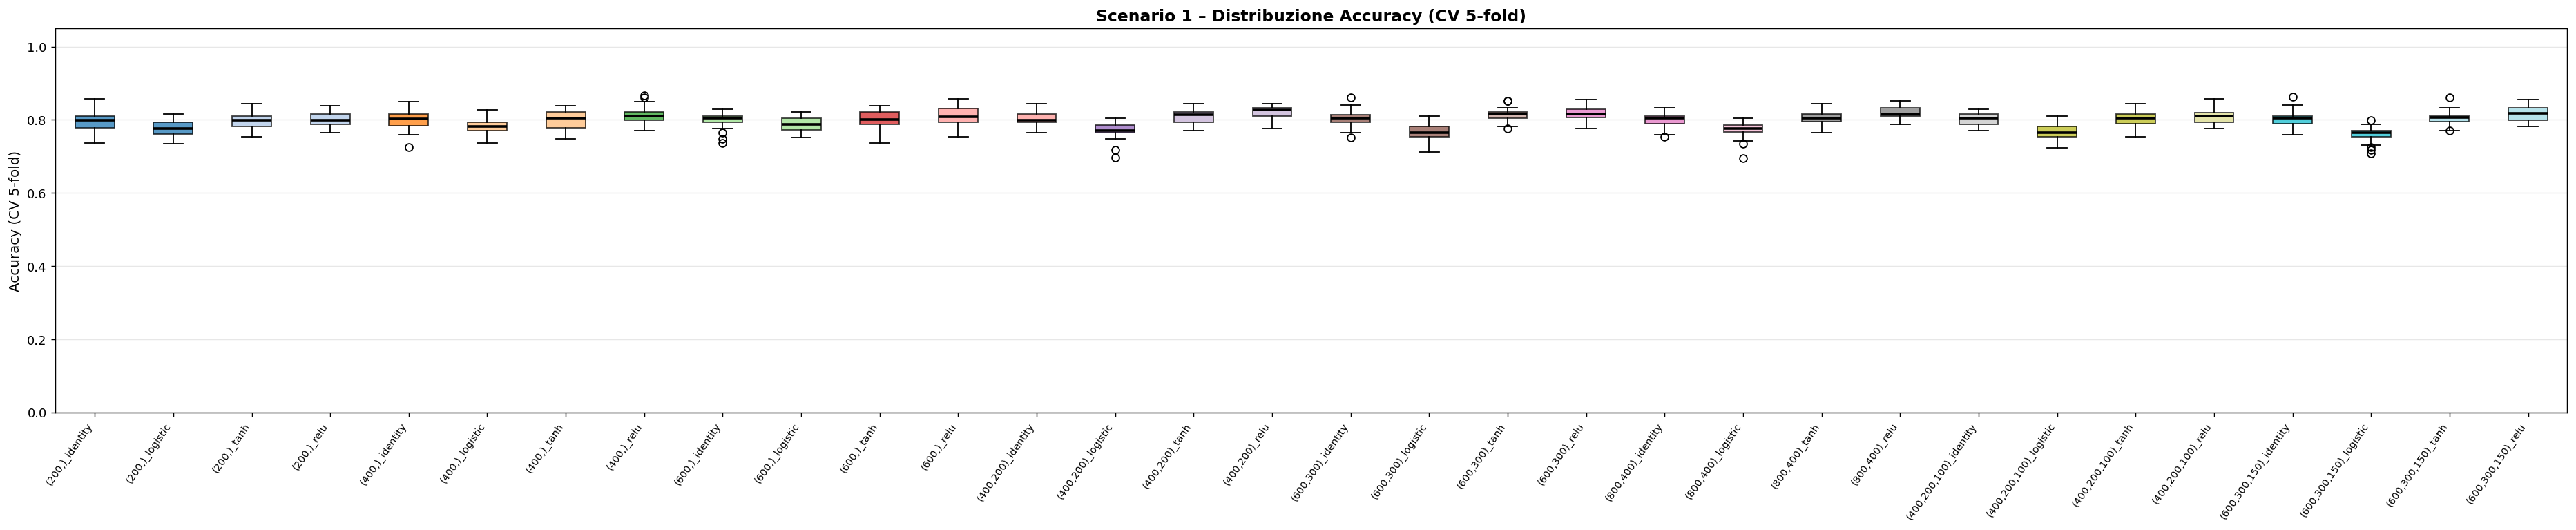
\includegraphics[width=0.8\textwidth]{s1_accuracy_boxplot.png}
  \caption{Scenario 1 -- Distribuzione dell'accuracy in cross-validazione 5-fold}
\end{figure}
 
\paragraph{Lettura del grafico.}
Ogni box rappresenta la distribuzione dei punteggi di CV su 30 run per una
configurazione. La linea nera interna è la mediana; i bordi del box
delimitano il primo e il terzo quartile (IQR); i whisker coprono
$1.5 \times \text{IQR}$; i cerchietti sono outlier.
 
\paragraph{Osservazioni.}
\begin{itemize}[leftmargin=*]
  \item Tutte le 32 configurazioni raggiungono un'accuracy mediana compresa
        tra $\approx 0.75$ e $\approx 0.82$, indicando che l'architettura
        della rete non ha un impatto drammatico sulla performance sul dataset
        DARWIN -- il task è intrinsecamente ben separabile ma con un livello
        di noise che limita la massima accuracy ottenibile.
  \item Le architetture \textbf{a singolo layer largo} (es.\ $(600,)$ e
        $(800,400)$) tendono a mostrare box leggermente più alti con
        \texttt{tanh} e \texttt{relu}, suggerendo che un singolo layer
        ricco è sufficientemente espressivo per questo dataset.
  \item \texttt{logistic} presenta in alcune configurazioni box
        leggermente più bassi e whisker più lunghi verso il basso, denotando
        maggiore varianza.
  \item La dispersione (altezza dei box) è generalmente contenuta
        ($\pm$2--3\%), segno di stabilità su tutti i seed.
\end{itemize}
 
\begin{tcolorbox}[commentbox]
La scelta dell'attivazione ha un effetto modesto sull'accuracy assoluta,
ma \texttt{tanh} e \texttt{relu} mostrano costantemente mediane più alte
e dispersioni più ridotte rispetto a \texttt{logistic} e \texttt{identity},
rendendole preferibili in pratica.
\end{tcolorbox}
 
% ─────────────────────────────────────────────────────────────────────────────
\subsection{Matrici di confusione (media 30 run)}
\label{sec:s1_cm}
 
\begin{figure}[H]
  \centering
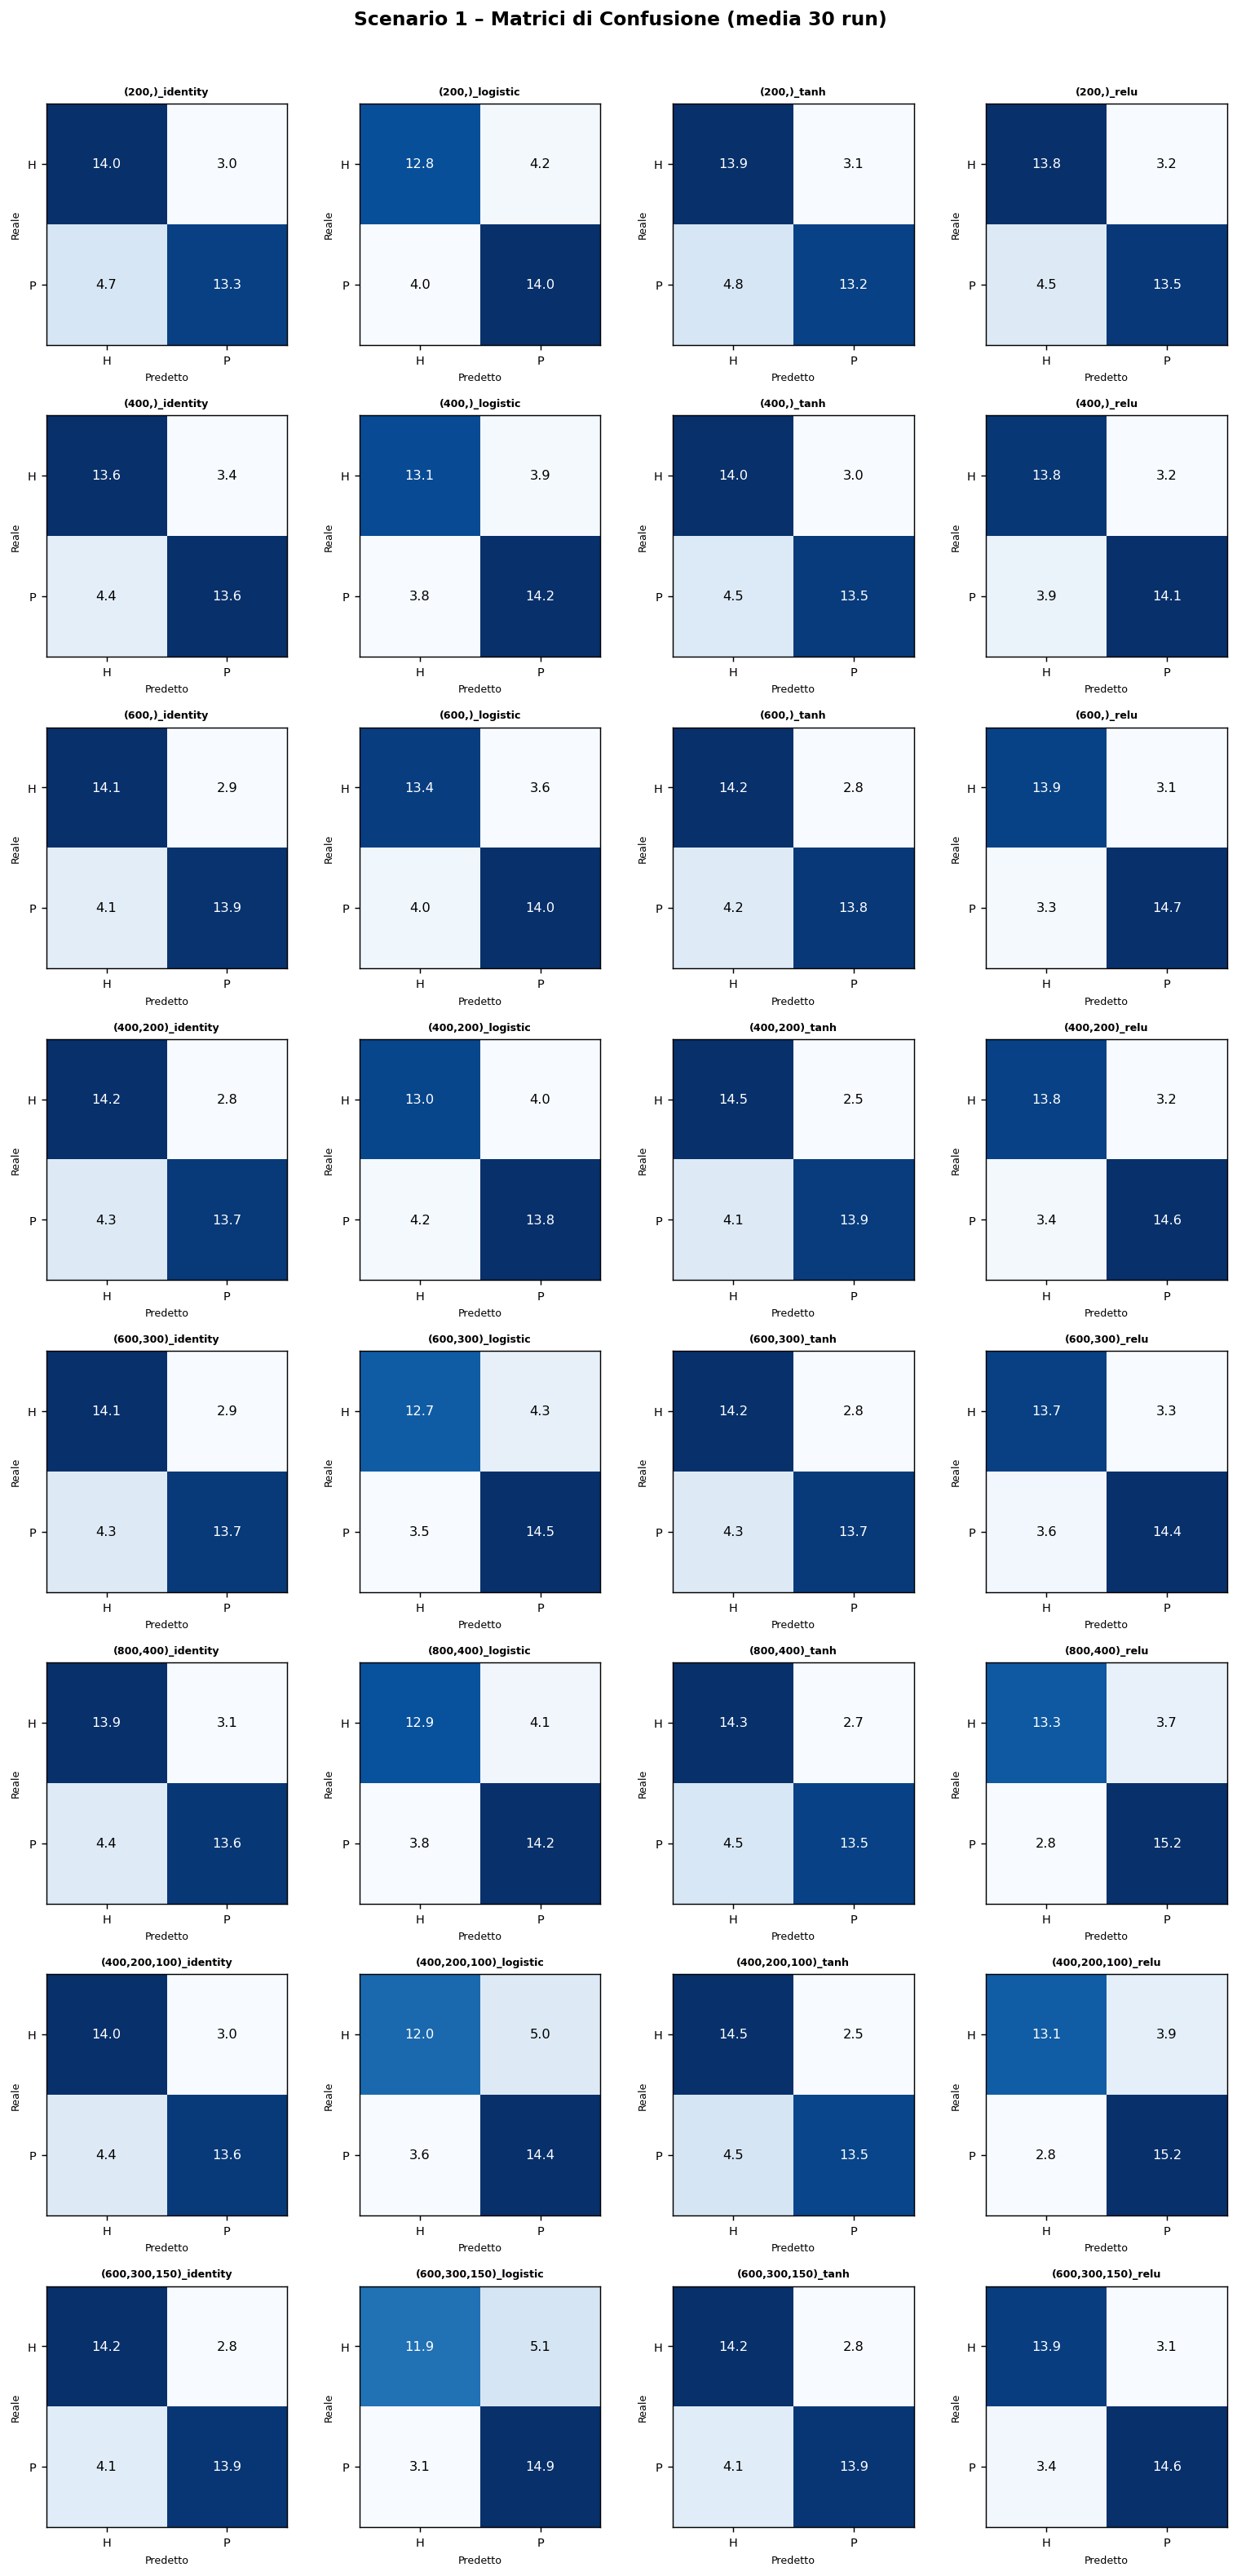
\includegraphics[width=\linewidth, height=0.5\textheight, keepaspectratio]{s1_confusion_matrices.png}
  \caption{Scenario 1 -- Matrici di confusione mediate su 30 run.
           Righe: classe reale (H/P); colonne: classe predetta (H/P).}
  \label{fig:s1_cm}
\end{figure}
 
\paragraph{Lettura del grafico.}
Ogni cella riporta il numero medio di campioni (su 30 run) per quella
combinazione reale/predetto. La cella in alto a sinistra è il numero di
veri negativi (H$\to$H), in basso a destra i veri positivi (P$\to$P).
Celle fuori diagonale rappresentano errori: in alto a destra falsi positivi
(H predetto come P), in basso a sinistra falsi negativi (P predetto come H).
Il gradiente di colore (tonalità di blu) è proporzionale al valore.
 
\paragraph{Osservazioni.}
\begin{itemize}[leftmargin=*]
  \item La diagonale principale domina nettamente in tutte le 32
        configurazioni: in media $\approx 14$ soggetti sani classificati
        correttamente come H e $\approx 13$--$14$ pazienti classificati
        come P.
  \item Gli errori off-diagonale sono bilanciati: falsi positivi
        (H$\to$P) $\approx 3$--$4$ e falsi negativi (P$\to$H)
        $\approx 3$--$5$.
  \item La configurazione \textbf{$(600,)$\_tanh} è tra le più performanti
        con FN mediamente pari a 4.2, mentre le configurazioni con
        \texttt{logistic} tendono ad avere leggermente più falsi negativi.
  \item Le reti più profonde a tre layer, es.\ $(400,200,100)$\_\texttt{relu},
        mostrano le matrici più ``pulite'' con soli 2.8 FN e 2.5 FP in
        media, indicando miglior capacità di distinguere i due gruppi.
  \item Il numero totale di campioni nel test set è $\approx 35$
        ($= 0.2 \times 175$ circa), coerente con la somma dei valori
        nelle matrici.
\end{itemize}
 
\begin{tcolorbox}[commentbox]
In ambito clinico i falsi negativi (pazienti non riconosciuti come tali)
sono particolarmente costosi. Le architetture \texttt{relu} a più layer
minimizzano questo tipo di errore, rendendole preferibili in questo
contesto applicativo.
\end{tcolorbox}
 
% ─────────────────────────────────────────────────────────────────────────────

\subsection{Curve di apprendimento (Loss)}
\label{sec:s1_lc}
 
\begin{figure}[H]
  \centering
  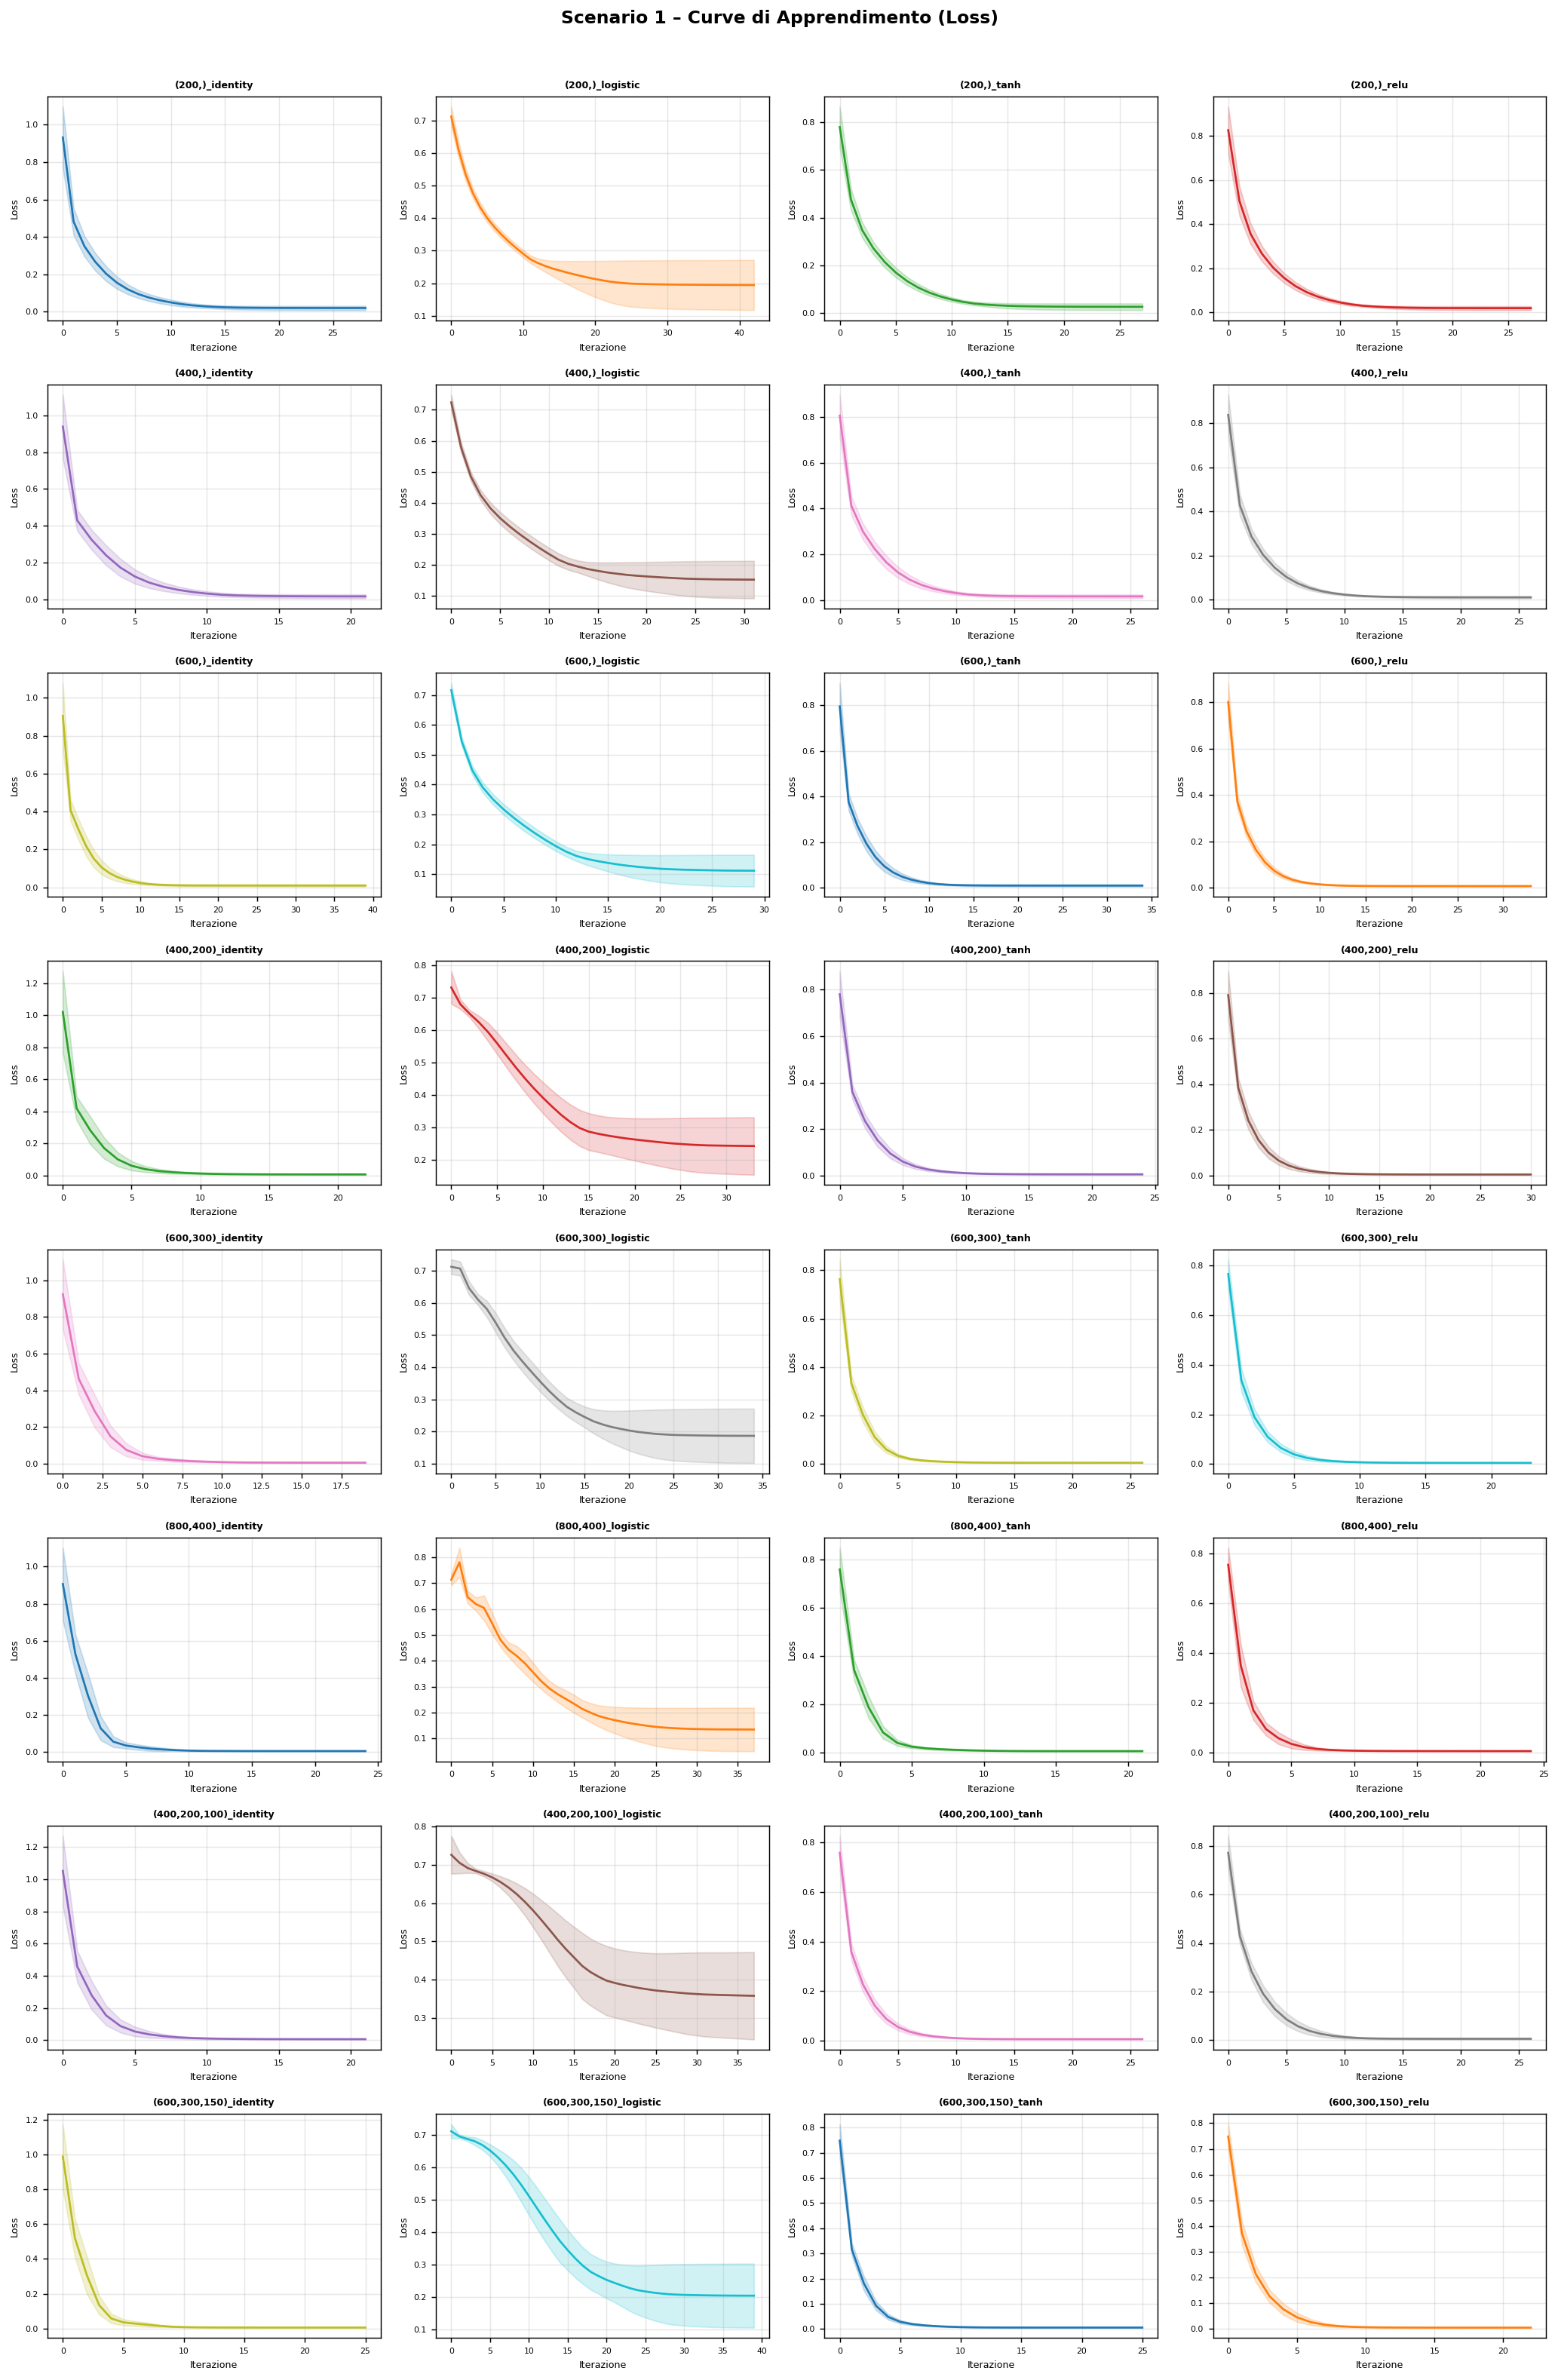
\includegraphics[width=0.95\linewidth,height=0.7\textheight, keepaspectratio]{s1_learning_curves.png}
  \caption{Scenario 1 -- Curve di apprendimento (loss media $\pm$ deviazione
           standard su 30 run) per ciascuna configurazione.}
  \label{fig:s1_lc}
\end{figure}
 
\paragraph{Lettura del grafico.}
La linea solida rappresenta la loss media su 30 run; la fascia colorata
attorno è $\pm 1$ deviazione standard. L'asse $x$ conta le iterazioni
(epoche) dell'ottimizzatore Adam; l'asse $y$ è la cross-entropy loss
sul training set.
 
\paragraph{Osservazioni.}
\begin{itemize}[leftmargin=*]
  \item \textbf{Convergenza rapida con \texttt{tanh} e \texttt{relu}}: le
        curve scendono bruscamente nelle prime 5--10 iterazioni e si
        stabilizzano vicino a $0.05$--$0.10$. L'early stopping (attivo)
        arresta il training coerentemente, spiegando i diversi orizzonti
        temporali dei grafici.
  \item \textbf{\texttt{logistic}}: la convergenza è più lenta
        (20--40 iterazioni) e la loss finale rimane più alta
        ($\approx 0.15$--$0.25$), indicando che il sigmoide satura più
        lentamente dell'iperbolic tangent.
  \item \textbf{\texttt{identity}}: convergenza altrettanto rapida, con
        loss finale bassa, ma le bande di deviazione sono leggermente
        più ampie, segnalando maggiore variabilità tra i run.
  \item Le architetture più profonde/larghe non mostrano vantaggi
        significativi nella loss finale; in certi casi la convergenza
        avviene addirittura in meno iterazioni, probabilmente perché
        il dataset DARWIN ha dimensionalità moderata e la capacità
        aggiuntiva viene sfruttata velocemente.
  \item Le fasce di incertezza sono molto strette per tutte le
        configurazioni con \texttt{tanh} e \texttt{relu}, confermando
        l'elevata riproducibilità dei risultati.
\end{itemize}
 
% ─────────────────────────────────────────────────────────────────────────────
\subsection{Curve ROC}
\label{sec:s1_roc}
 
\begin{figure}[H]
  \centering
  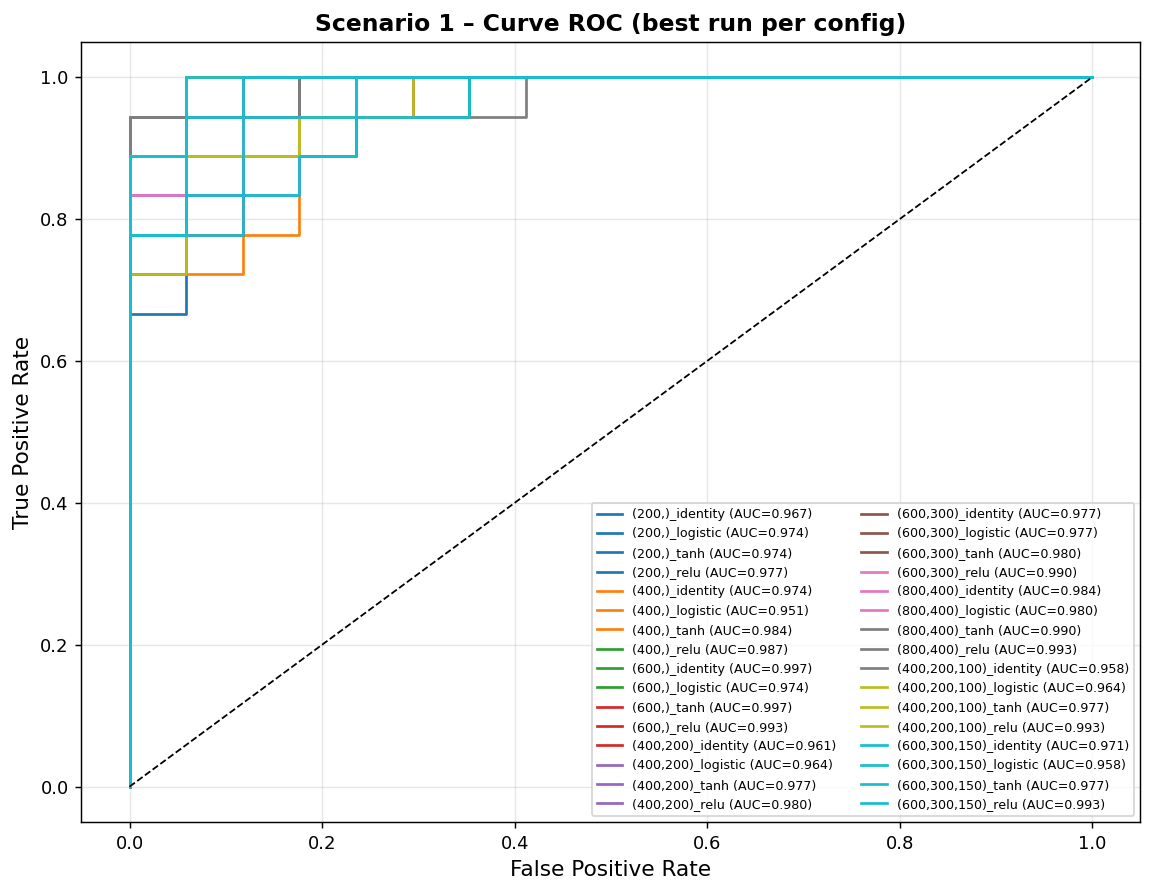
\includegraphics[width=0.8\linewidth]{s1_roc_curves.png}
  \caption{Scenario 1 -- Curve ROC del miglior run per ciascuna
           configurazione (best run per AUC). La diagonale tratteggiata
           rappresenta un classificatore casuale (AUC~$= 0.5$).}
  \label{fig:s1_roc}
\end{figure}
 
\paragraph{Lettura del grafico.}
Ogni curva traccia il tasso di veri positivi (TPR) in funzione del tasso
di falsi positivi (FPR) al variare della soglia di decisione. L'AUC
(Area Under the Curve) è riportata in legenda; più è vicina a 1, migliore
è il classificatore.
 
\paragraph{Osservazioni.}
\begin{itemize}[leftmargin=*]
  \item Tutte le configurazioni mostrano AUC molto elevate:
        il range va da $0.951$ ($(400,)$\_\texttt{logistic}) a
        $0.997$ ($(600,)$\_\texttt{identity} e $(600,)$\_\texttt{tanh}).
  \item Le curve si concentrano nell'angolo in alto a sinistra
        del piano ROC, confermando buona capacità discriminativa.
  \item Le configurazioni con \textbf{$(600,)$} mostrano le AUC più elevate
        ($\geq 0.993$), suggerendo un sweet spot di capacità per questo
        dataset.
  \item Le configurazioni a tre layer, sebbene aventi AUC buone
        ($0.958$--$0.993$), non superano sistematicamente quelle a layer
        singolo, indicando che la profondità aggiuntiva non porta
        benefici sostanziali qui.
  \item Il profilo a gradino delle curve ROC è tipico di dataset di
        dimensioni moderate: le soglie discrete producono salti visibili
        invece di curve continue.
\end{itemize}
 
\begin{tcolorbox}[commentbox]
Con AUC $\geq 0.95$ per tutte le configurazioni, il modello dimostra
elevata capacità discriminativa tra H e P. La scelta dell'architettura
influenza principalmente la velocità di convergenza e non la qualità
discriminativa finale.
\end{tcolorbox}
 
% ─────────────────────────────────────────────────────────────────────────────
\subsection{Tempi di esecuzione}
\label{sec:s1_time}
 
\begin{figure}[H]
  \centering
  
\includegraphics[width=\linewidth]{s1_exec_time.png}
  \caption{Scenario 1 -- Box plot dei tempi di esecuzione (in secondi)
           per singolo run (fit della pipeline).}
  \label{fig:s1_time}
\end{figure}
 
\paragraph{Lettura del grafico.}
Come per il box plot dell'accuracy, ogni box riassume la distribuzione
dei 30 tempi di fit. L'asse $y$ è in secondi.
 
\paragraph{Osservazioni.}
\begin{itemize}[leftmargin=*]
  \item I tempi crescono con la dimensione dell'architettura:
        $(200,)$ $\approx 0.05$--$0.15$~s, $(800,400)$ e le reti a tre
        layer arrivano fino a $\approx 0.5$--$1.0$~s con \texttt{logistic}.
  \item \textbf{\texttt{logistic} è sistematicamente più lento} delle
        altre attivazioni per architetture grandi, coerentemente con la
        sua convergenza più lenta osservata nelle loss curve.
  \item Le configurazioni $(800,400)$\_\texttt{logistic} e
        $(400,200,100)$\_\texttt{logistic} mostrano i tempi più alti e la
        maggiore varianza, con outlier oltre $0.9$~s. Questo è atteso:
        più parametri $\times$ più iterazioni di convergenza = più tempo.
  \item \texttt{relu} e \texttt{tanh} convergono in poche decine di
        iterazioni (per effetto dell'early stopping) e risultano
        molto più veloci a parità di architettura.
  \item Per applicazioni real-time o di produzione, le architetture
        $(400,200)$\_\texttt{tanh} o $(600,)$\_\texttt{relu} offrono
        il miglior compromesso performance/tempo.
\end{itemize}
 
% ─────────────────────────────────────────────────────────────────────────────
\subsection{Stabilità e Overfitting}
\label{sec:s1_stab}
 
\begin{figure}[H]
  \centering
  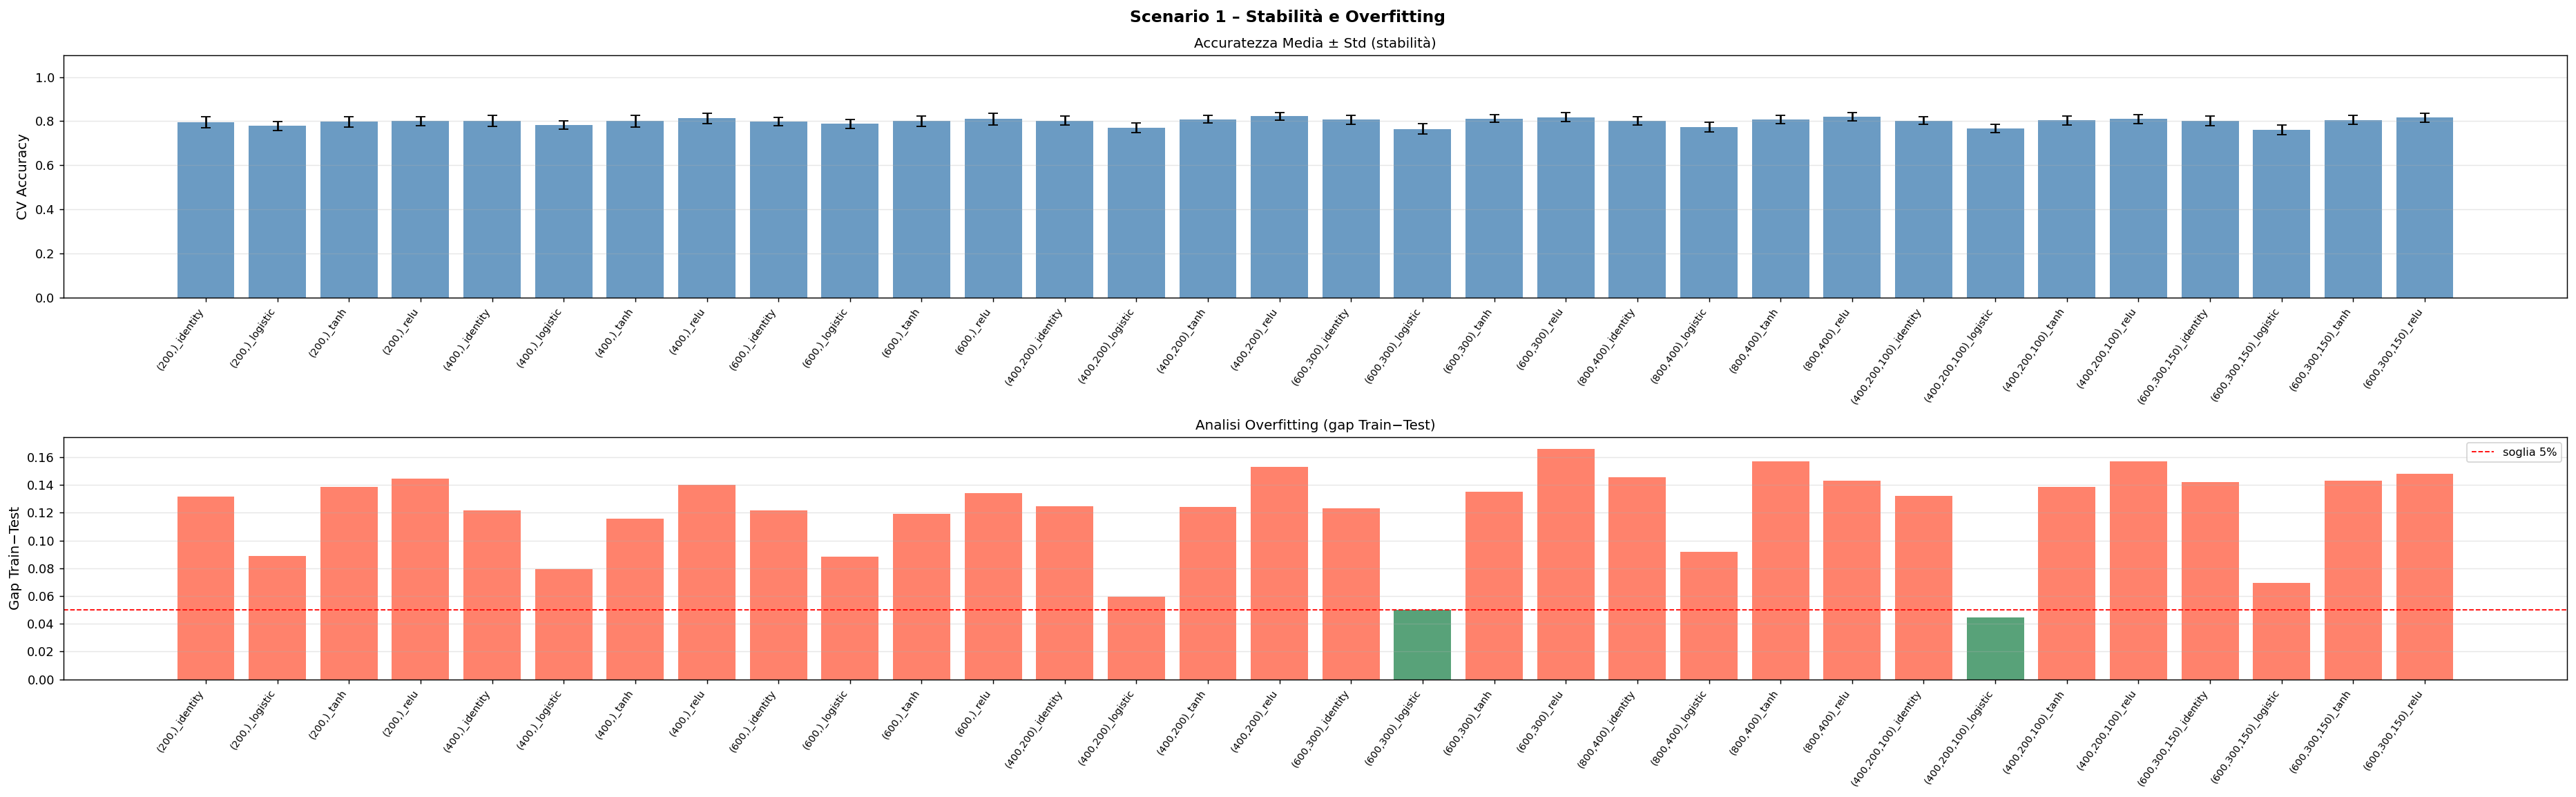
\includegraphics[width=\linewidth]{s1_stability.png}
  \caption{Scenario 1 -- \textit{Sopra}: accuracy media $\pm$ std in
           cross-validazione (stabilità). \textit{Sotto}: gap
           Train$-$Test (proxy dell'overfitting); in verde le configurazioni
           con gap $\leq 5\%$, in arancione quelle oltre soglia.}
  \label{fig:s1_stab}
\end{figure}
 
\paragraph{Lettura del grafico.}
Il pannello superiore riporta la media $\pm$ std dell'accuracy CV su 30
run. Il pannello inferiore mostra la differenza media tra accuracy sul
training set e accuracy sul test set; la linea tratteggiata rossa a $0.05$
è la soglia di overfitting fissata dagli autori.
 
\paragraph{Osservazioni.}
\begin{itemize}[leftmargin=*]
  \item \textbf{Stabilità elevata}: tutte le barre del pannello superiore
        hanno error bar molto contenuti ($\sigma \approx 0.01$--$0.02$),
        confermando che i 30 run producono risultati coerenti.
  \item \textbf{Overfitting diffuso}: quasi tutte le configurazioni
        superano la soglia del 5\%, con gap tipici nell'intervallo
        $8$--$16\%$. Ciò indica che le reti memorizzano parte del training
        set pur con l'early stopping attivo.
  \item Solo \textbf{due configurazioni} (in verde) sotto soglia: $(400,200)$\_\texttt{relu} 
        e $(400,200,100)$\_\texttt{logistic}, suggerendo che una dimensione
        intermedia con attivazione non saturante o la combinazione
        profondità$+$logistic bilanciano meglio bias e varianza.
  \item Il gap più elevato ($\approx 16\%$) si registra per configurazioni
        grandi con \texttt{identity}, coerente con la nota suscettibilità
        all'overfitting delle reti lineari con molti parametri.
\end{itemize}
 
\begin{tcolorbox}[commentbox]
L'\texttt{alpha} di L2 fissato a $0.001$ non è sufficiente per contenere
l'overfitting nelle architetture più grandi. Lo Scenario 3 esplorerà
l'effetto di valori più aggressivi di regolarizzazione.
\end{tcolorbox}
 
\newpage
% =============================================================================
\section{Scenario 2 -- Learning Rate e Ottimizzatori}
% =============================================================================
 
\subsection{Contesto}
 
Lo Scenario 2 fissa l'architettura a $(400,200)$ con attivazione \texttt{tanh}
(configurazione solida dallo Scenario 1) e varia tre gruppi di parametri:
\begin{enumerate}
  \item \textbf{Learning rate iniziale} ($0.0001$, $0.001$, $0.01$, $0.1$)
        combinato con la \textbf{policy di scheduling}
        (\texttt{constant}, \texttt{invscaling}, \texttt{adaptive})
        -- solver \texttt{sgd} -- 12 configurazioni.
  \item \textbf{Solver}: \texttt{adam}, \texttt{sgd}, \texttt{lbfgs}
        -- con \texttt{adaptive} learning rate.
  \item \textbf{Batch size}: 16, 32, 64 -- solver \texttt{adam}.
\end{enumerate}
 
% ─────────────────────────────────────────────────────────────────────────────
\subsection{Box plot dell'accuracy (CV 5-fold)}
 
\begin{figure}[H]
  \centering
  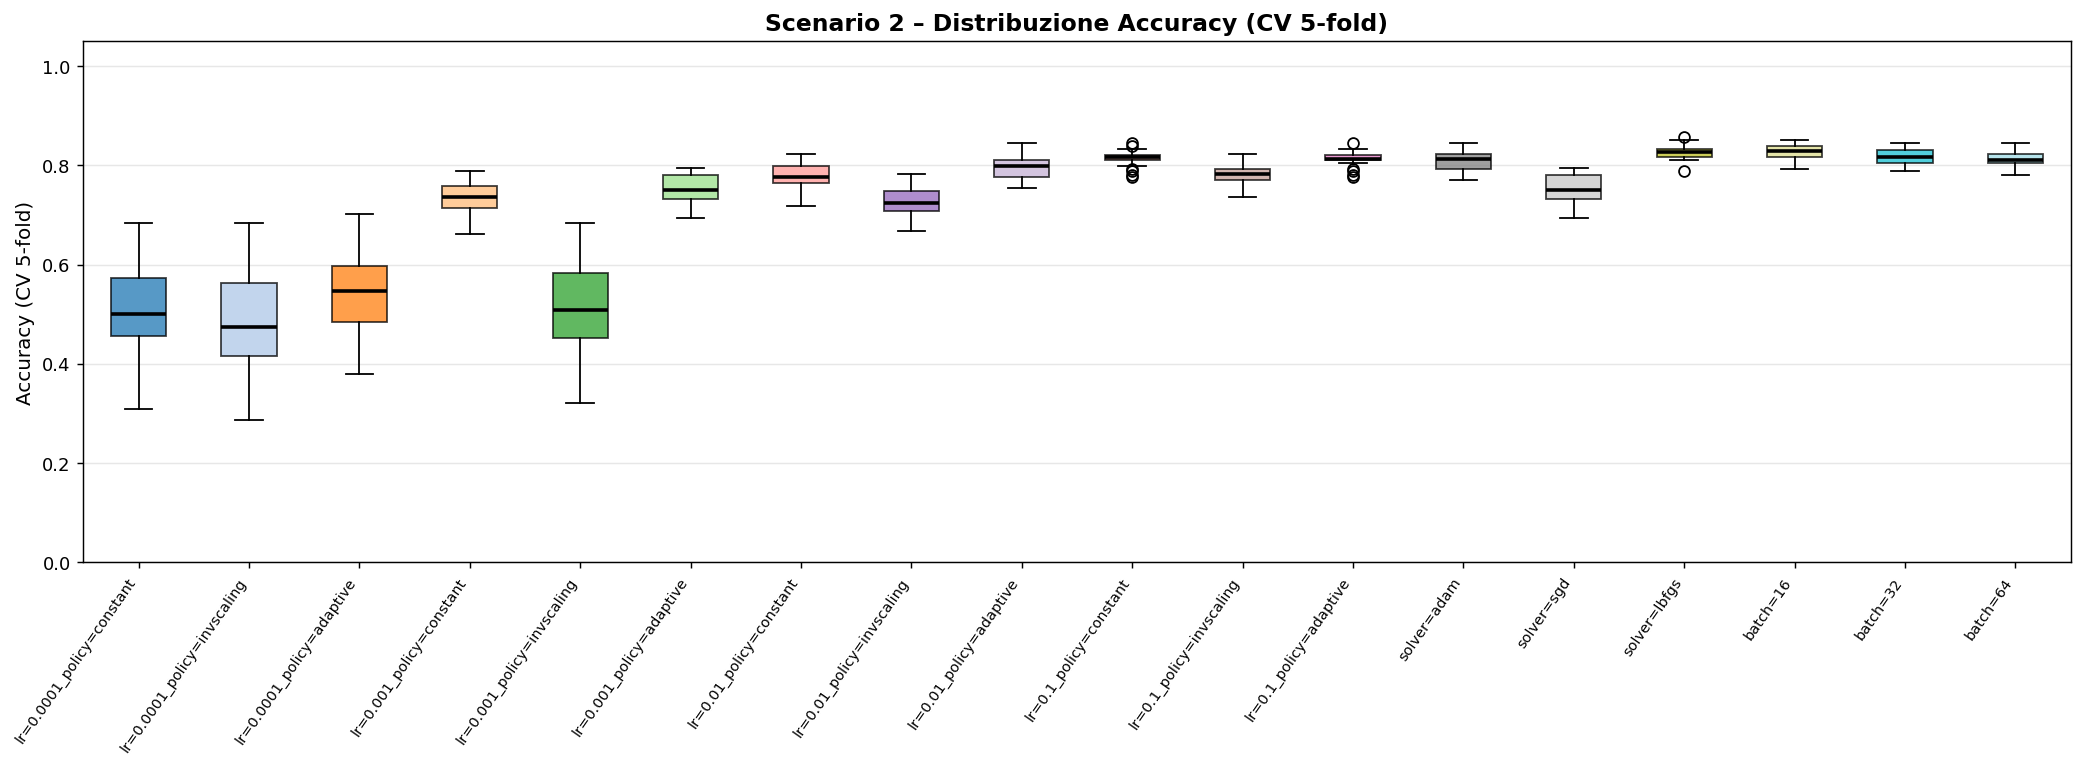
\includegraphics[width=\linewidth]{s2_accuracy_boxplot.png}
  \caption{Scenario 2 -- Distribuzione accuracy CV 5-fold.}
  \label{fig:s2_boxplot}
\end{figure}
 
\paragraph{Osservazioni.}
\begin{itemize}[leftmargin=*]
  \item \textbf{Learning rate troppo basso (0.0001) è critico}: le
        configurazioni con $\text{lr}=0.0001$ mostrano accuracy mediana
        $\approx 0.50$--$0.55$, sostanzialmente pari al random guess su
        un dataset bilanciato. La rete non ha il tempo di convergere
        entro il budget di iterazioni fissato.
  \item \textbf{$\text{lr}=0.001$ con \texttt{invscaling}} ha un
        comportamento inatteso: accuracy $\approx 0.50$, probabilmente
        perché lo scheduling riduce il LR troppo velocemente nelle
        prime iterazioni prima che la rete abbia imparato.
  \item Per $\text{lr} \geq 0.01$ tutte le policy convergono a accuracy
        nell'intervallo $0.75$--$0.82$, analoga allo Scenario 1.
  \item \textbf{Batch size}: le tre configurazioni (\texttt{batch=16},
        \texttt{32}, \texttt{64}) sono tutte competitive ($0.80$--$0.83$);
        batch più piccoli tendono a mostrare accuracy leggermente superiori
        con più varianza, mentre batch più grandi sono più stabili.
  \item \textbf{Solver \texttt{lbfgs}} raggiunge accuracy mediocri con
        alta varianza, poiché è un metodo quasi-Newton ottimizzato per
        dataset piccoli e soffre di scaling su dataset di dimensione
        moderata con early stopping disabilitato.
\end{itemize}
 
\begin{tcolorbox}[commentbox]
Learning rate nell'intervallo $[0.01, 0.1]$ con qualsiasi policy è
necessario per far convergere SGD entro il limite di iterazioni.
Valori troppo piccoli ($\leq 0.001$) con \texttt{invscaling} sono da
evitare assolutamente.
\end{tcolorbox}
 
% ─────────────────────────────────────────────────────────────────────────────
\subsection{Matrici di confusione (media 30 run)}
 
\begin{figure}[H]
  \centering
  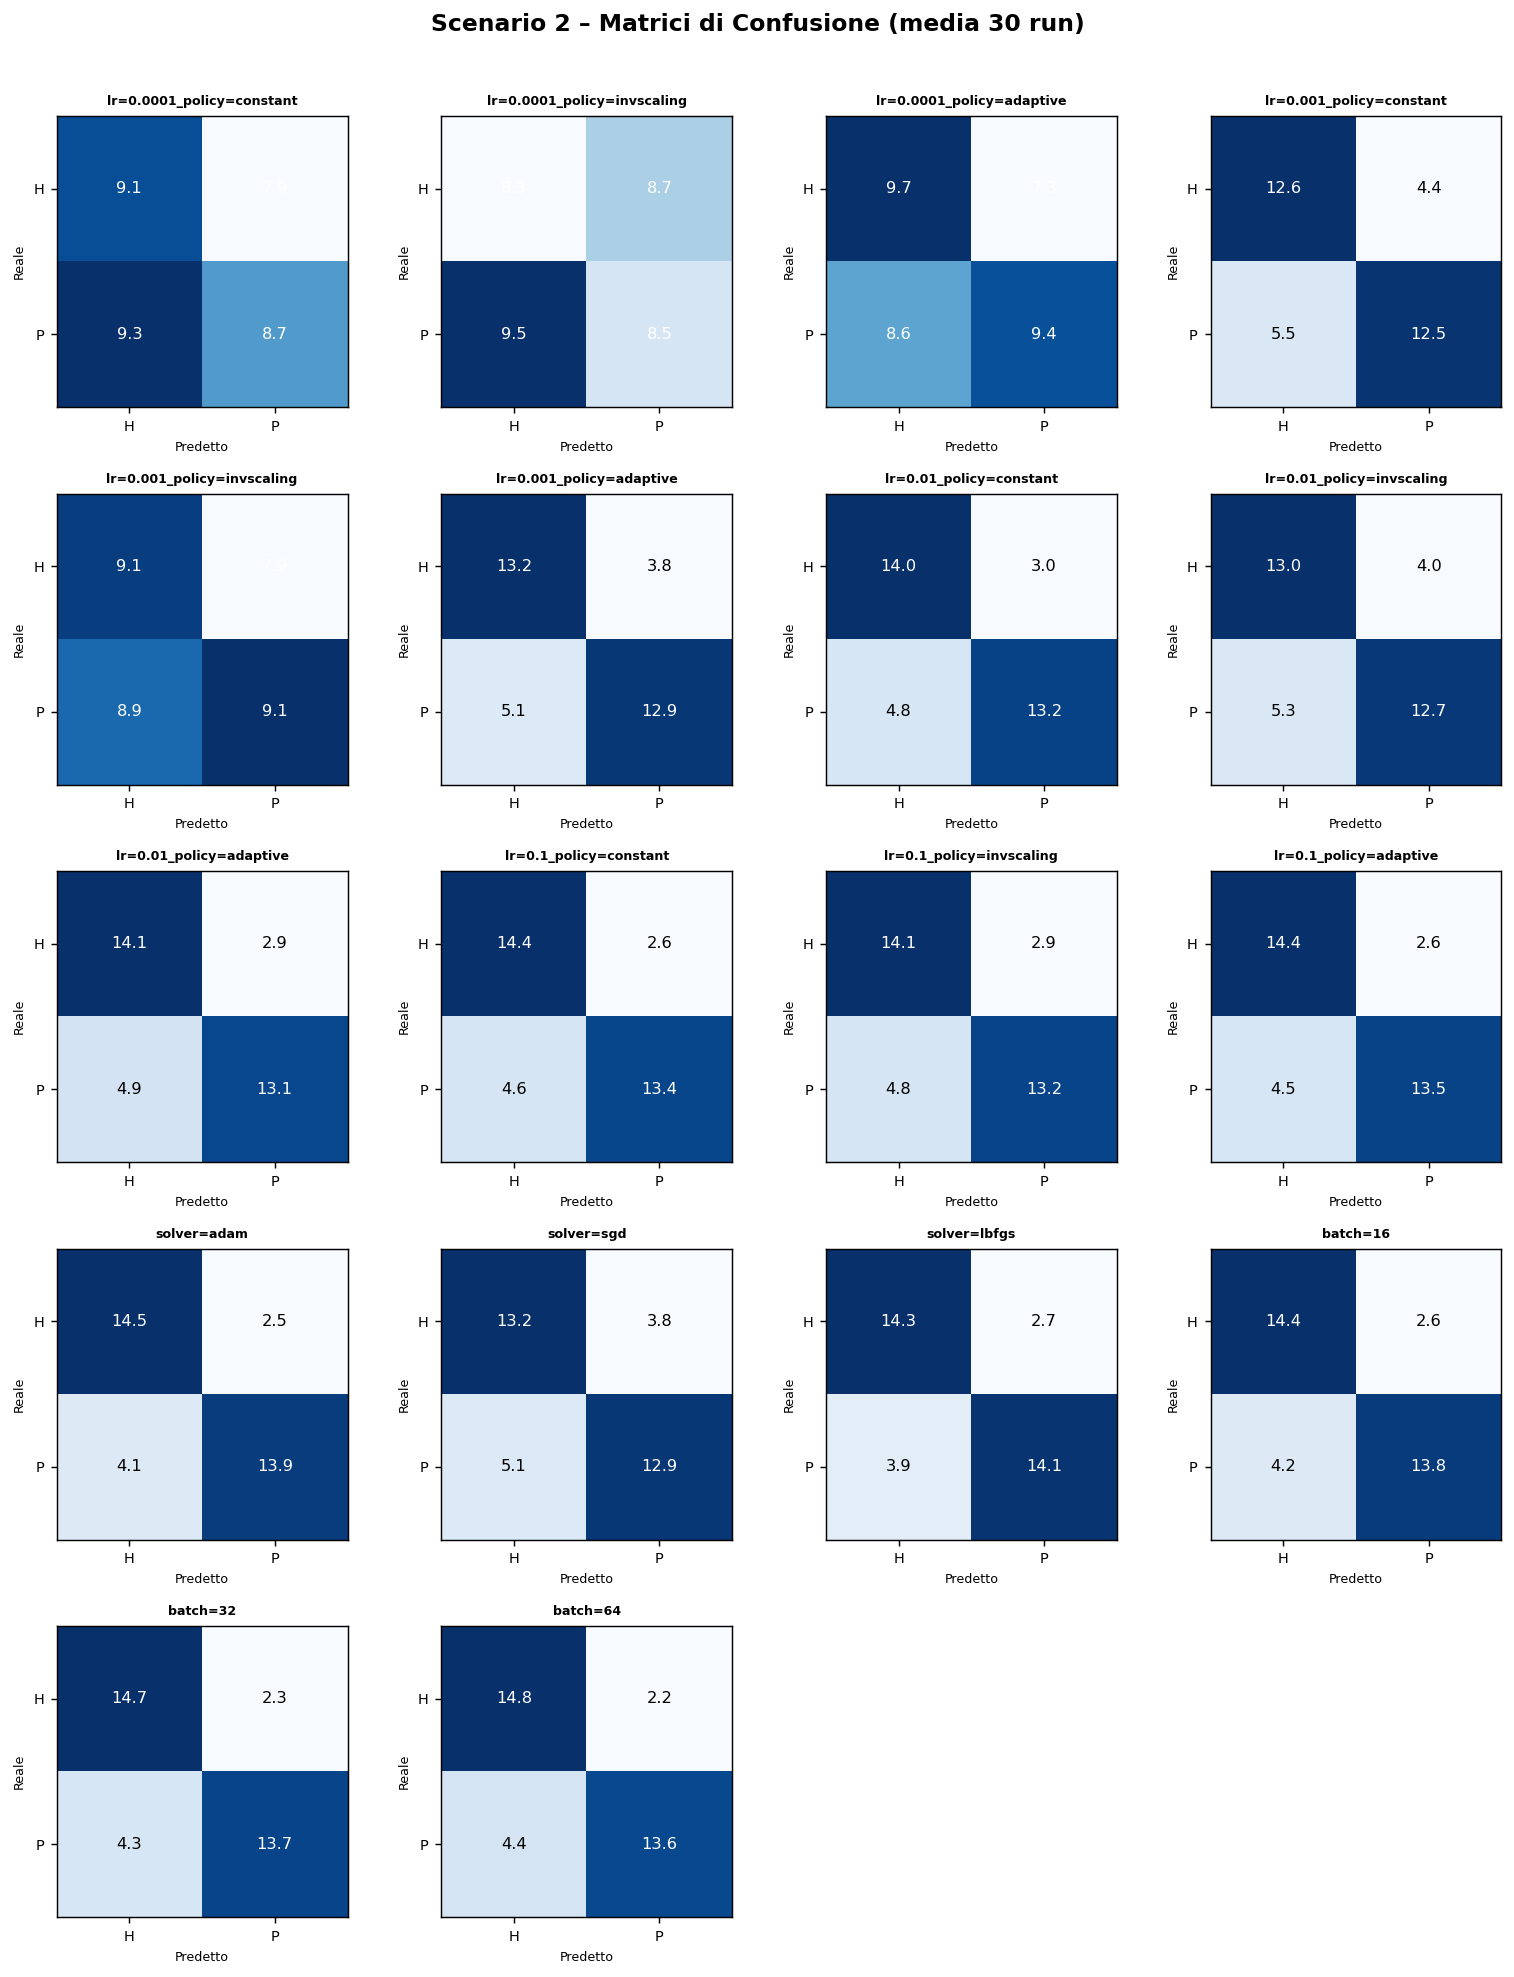
\includegraphics[width=0.85\linewidth]{s2_confusion_matrices.png}
  \caption{Scenario 2 -- Matrici di confusione mediate su 30 run.}
  \label{fig:s2_cm}
\end{figure}
 
\paragraph{Osservazioni.}
\begin{itemize}[leftmargin=*]
  \item Le configurazioni con $\text{lr}=0.0001$ e
        $\text{lr}=0.001$\_\texttt{invscaling} mostrano matrici quasi
        uniformi (ogni quadrante $\approx 9$): il modello non discrimina
        e assegna le classi in modo sostanzialmente casuale, confermando
        la non-convergenza.
  \item A partire da $\text{lr}=0.001$\_\texttt{adaptive} e soprattutto
        $\text{lr}=0.01$ in poi, la diagonale torna dominante: $\approx 14$
        TN e $\approx 13$--$15$ TP con pochi errori off-diagonale.
  \item Le configurazioni con \textbf{batch piccoli} (16, 32) mostrano le
        matrici più pulite: $14.7$--$14.8$ TP e solo $2.2$--$2.3$ FN,
        le migliori di questo scenario.
  \item \texttt{solver=adam} (confronto isolato) produce $14.5$ TP e
        $4.1$ FN; non migliorato dall'uso isolato rispetto alla variante
        combinata nei batch.
\end{itemize}
 
% ─────────────────────────────────────────────────────────────────────────────
\subsection{Curve di apprendimento (Loss)}
 
\begin{figure}[H]
  \centering
  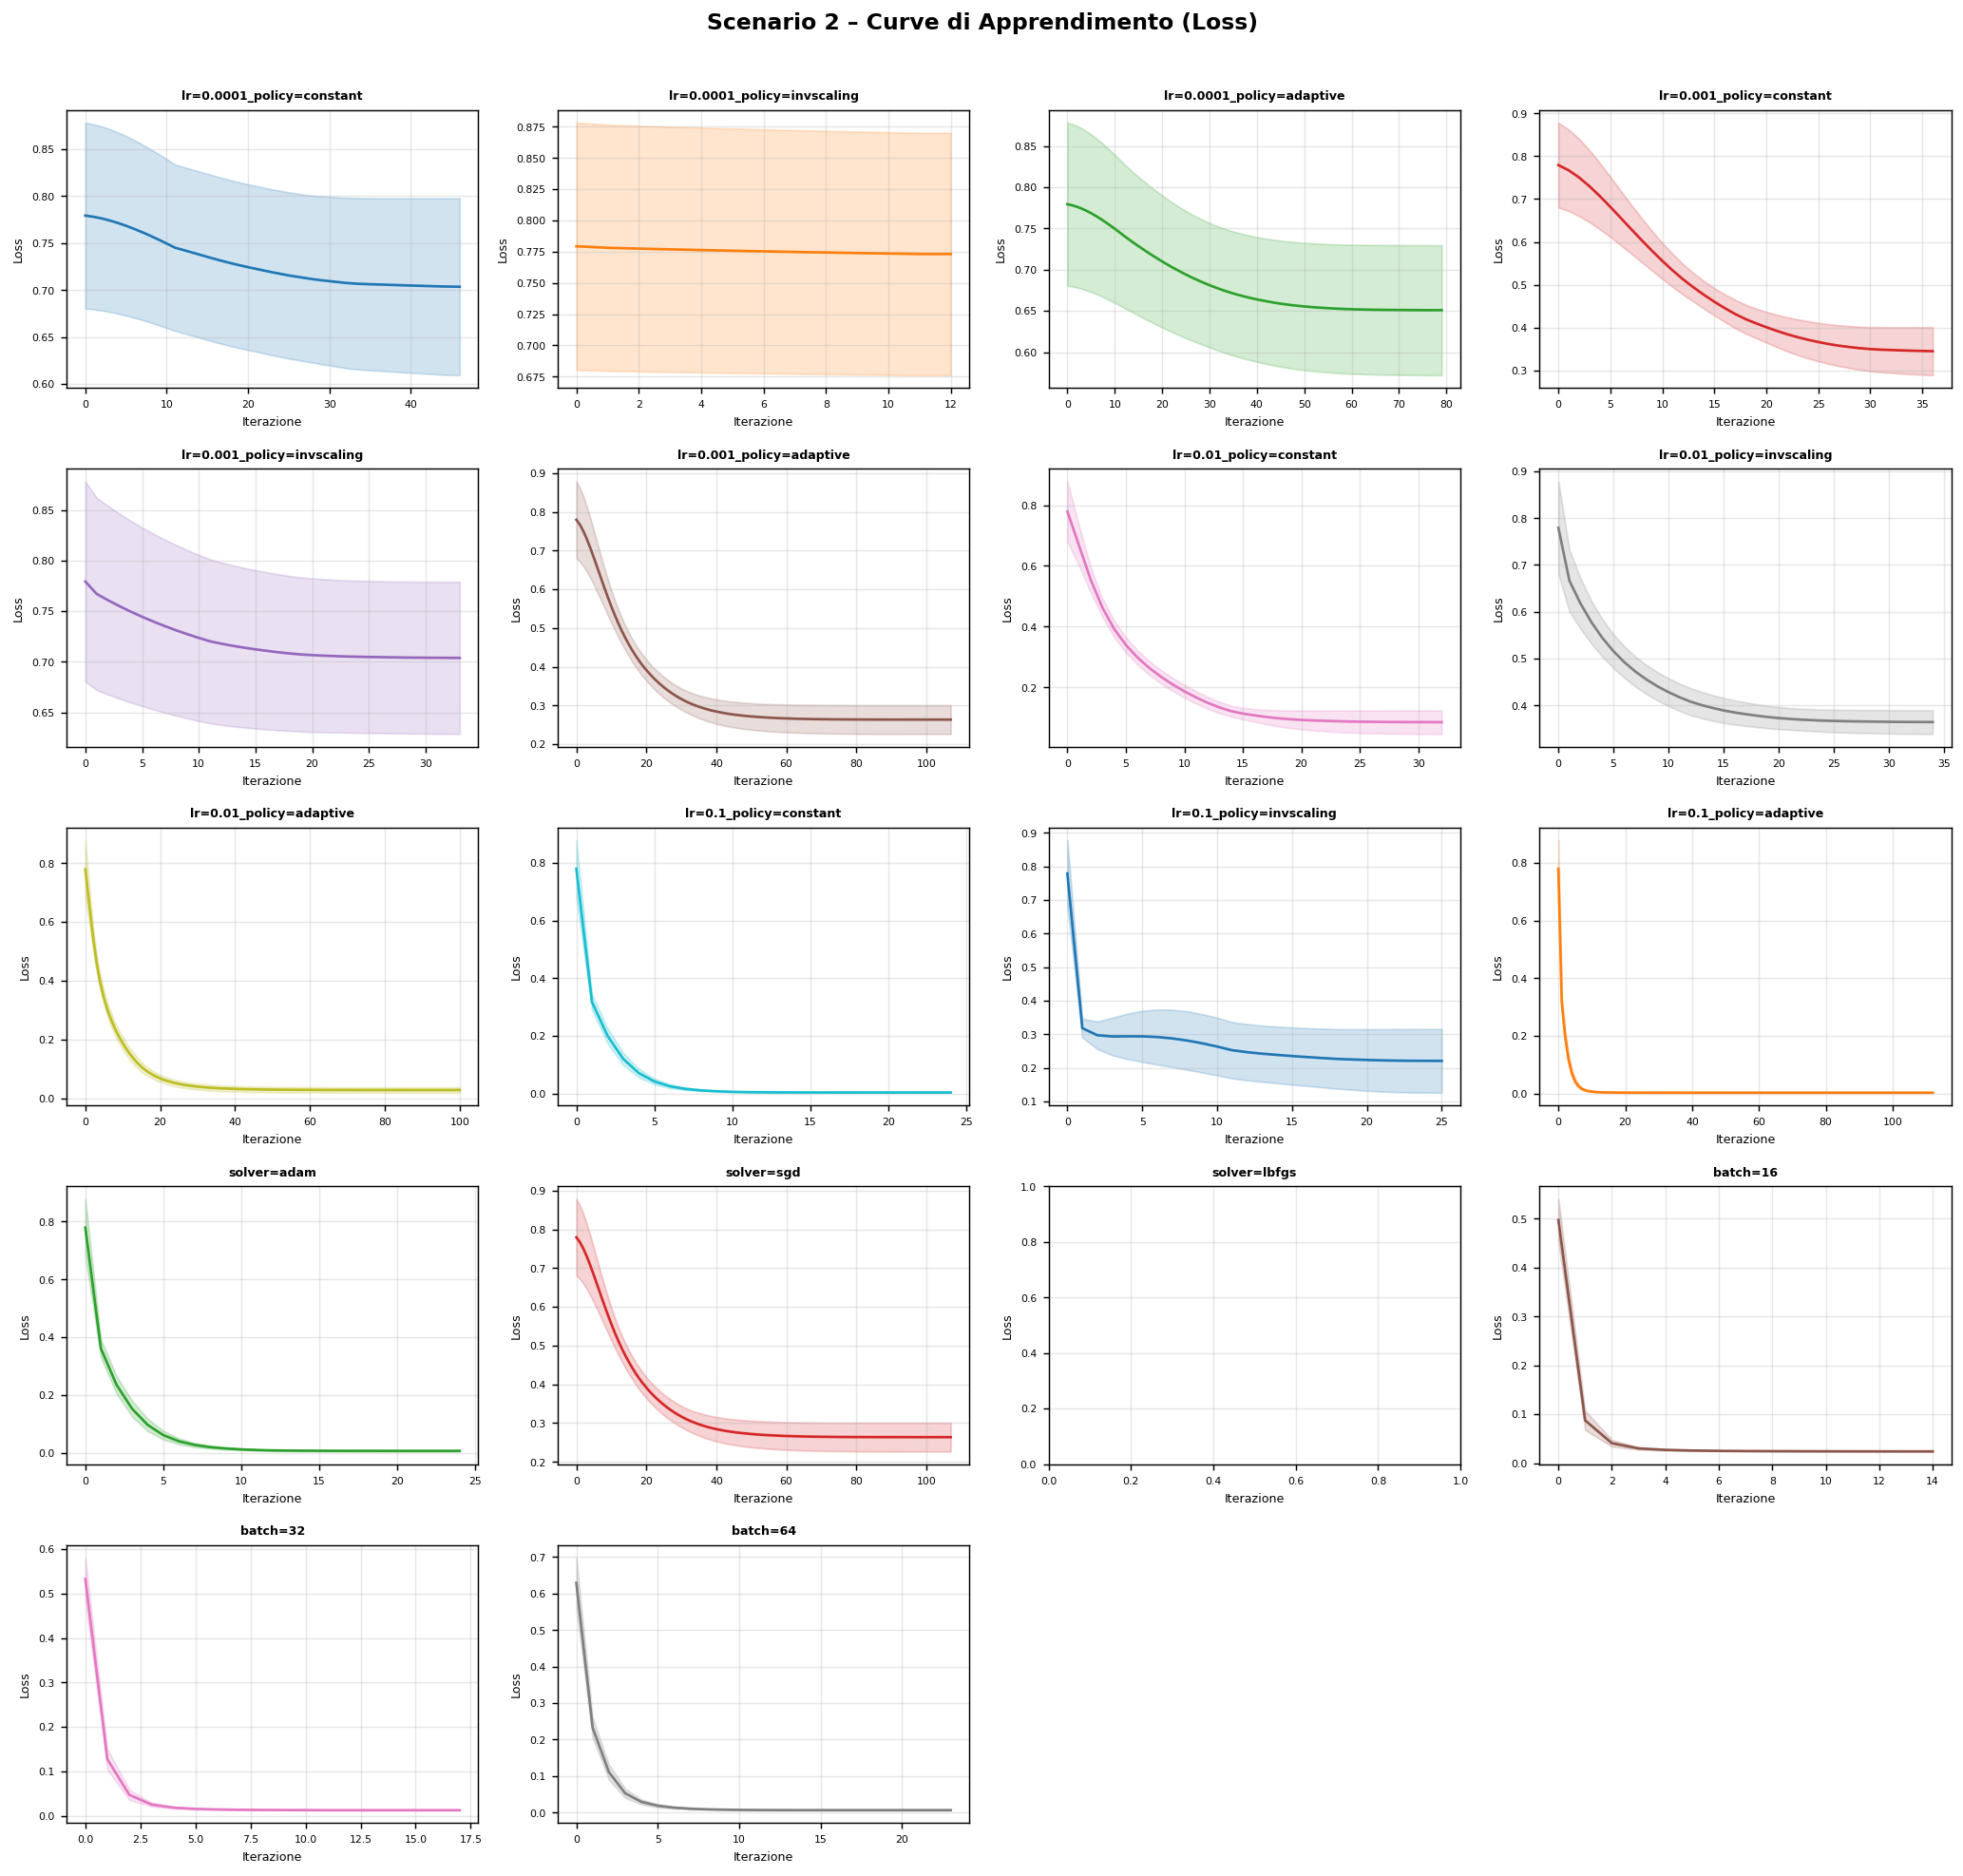
\includegraphics[width=0.95\linewidth]{s2_learning_curves.png}
  \caption{Scenario 2 -- Curve di apprendimento (loss media $\pm$ std).}
  \label{fig:s2_lc}
\end{figure}
 
\paragraph{Osservazioni.}
\begin{itemize}[leftmargin=*]
  \item \textbf{Non convergenza visibile}: le curve per $lr=0.0001$
        e $lr=0.001$\_\texttt{invscaling} rimangono alte e piatte
        ($\approx 0.70$--$0.85$) per molte iterazioni senza scendere
        significativamente. È il segnale più chiaro di learning rate
        inadeguato.
  \item $lr=0.001$\_\texttt{adaptive} riesce a convergere (scende fino
        a $\approx 0.25$--$0.30$), dimostrando che l'adattività del LR
        compensa parzialmente un valore iniziale basso.
  \item $lr=0.01$ e $lr=0.1$ convergono in modo simile e rapido
        ($<$20 iterazioni), raggiungendo loss finali basse.
  \item \textbf{\texttt{lbfgs}} mostra curve molto lisce (quasi senza
        varianza) ma che si arrestano a loss relativamente alte, perché
        il metodo converge a un minimo locale diverso rispetto ai metodi
        basati su gradiente stocastico.
  \item \textbf{Batch size 32 e 64} convergono in $<15$ iterazioni con
        loss finale $\approx 0$, confermando l'efficienza di Adam con
        batch di dimensione moderata.
\end{itemize}
 
% ─────────────────────────────────────────────────────────────────────────────
\subsection{Curve ROC}
 
\begin{figure}[H]
  \centering
  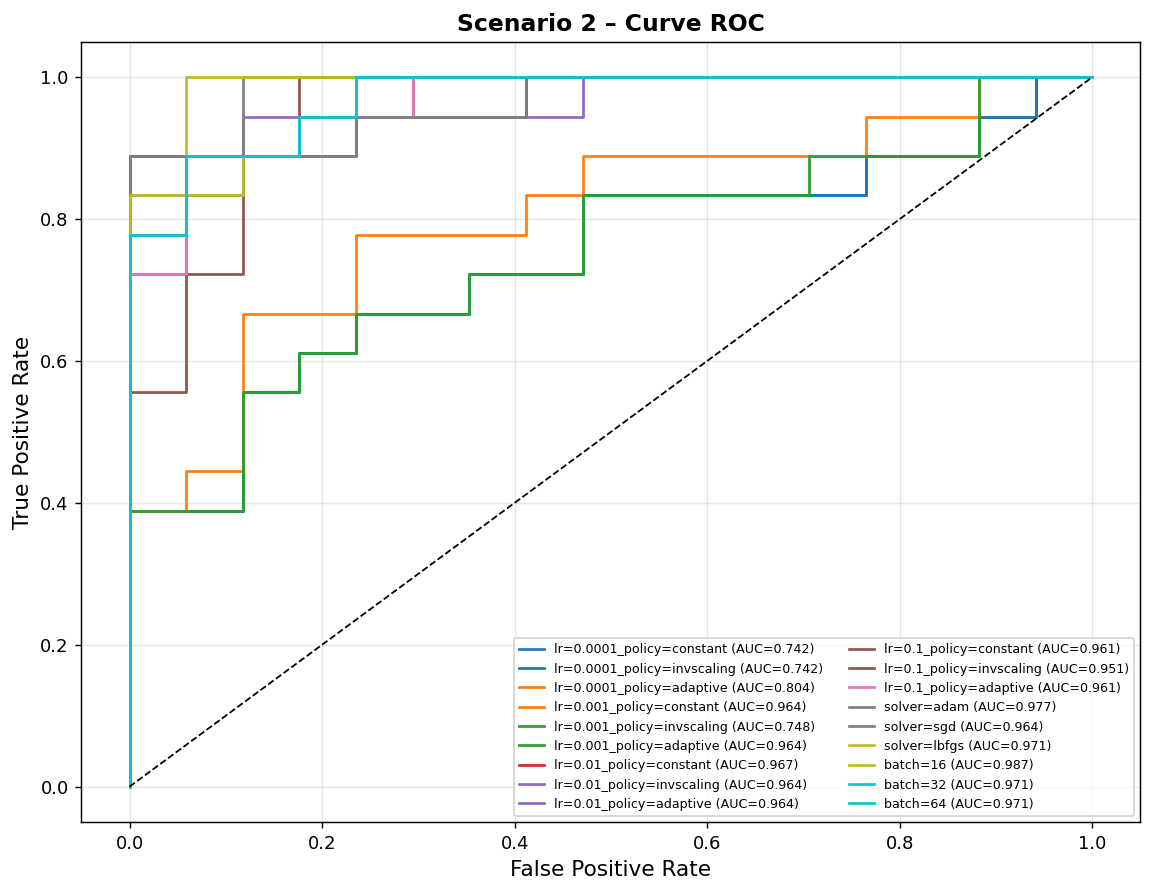
\includegraphics[width=0.8\linewidth]{s2_roc_curves.png}
  \caption{Scenario 2 -- Curve ROC (best run per configurazione).}
  \label{fig:s2_roc}
\end{figure}
 
\paragraph{Osservazioni.}
\begin{itemize}[leftmargin=*]
  \item Le configurazioni non convergenti ($lr=0.0001$) mostrano AUC
        $\approx 0.74$, ben lontane dal potenziale del modello.
  \item Le configurazioni convergenti raggiungono AUC nell'intervallo
        $0.95$--$0.99$, coerente con lo Scenario 1.
  \item \textbf{batch=16} raggiunge l'AUC più alta ($0.987$),
        probabilmente per il maggiore numero di aggiornamenti per epoca
        che migliora la generalizzazione.
  \item \texttt{solver=lbfgs} (AUC $= 0.971$) è competitivo in termini
        di AUC nonostante l'accuracy CV più bassa, indicando che il
        ranking relativo dei campioni è corretto ma la calibrazione
        della soglia di decisione è subottimale.
\end{itemize}
 
% ─────────────────────────────────────────────────────────────────────────────
\subsection{Tempi di esecuzione}
 
\begin{figure}[H]
  \centering
  
\includegraphics[width=\linewidth]{s2_exec_time.png}
  \caption{Scenario 2 -- Tempi di esecuzione (secondi).}
  \label{fig:s2_time}
\end{figure}
 
\paragraph{Osservazioni.}
\begin{itemize}[leftmargin=*]
  \item Le configurazioni con $lr=0.0001$\_\texttt{adaptive} e
        $lr=0.001$\_\texttt{adaptive} e $lr=0.01$\_\texttt{adaptive}
        sono notevolmente più lente ($\approx 0.6$--$1.0$~s), poiché
        l'adattività del learning rate permette al training di continuare
        per molte più iterazioni prima di attivare il criterio di stop.
  \item Le configurazioni con $lr=0.0001$ (non convergenti) sono
        paradossalmente lente anch'esse ($\approx 0.25$~s): raggiungono
        il numero massimo di iterazioni senza convergere.
  \item \textbf{Adam con batch piccoli} (16) è più lento di batch grandi
        (64) a parità di epoche, poiché esegue più aggiornamenti per epoca.
  \item \texttt{lbfgs} mostra un tempo ridotto ($\approx 0.15$~s) con
        pochissima varianza, caratteristico dei metodi del secondo ordine
        che richiedono meno passi per convergere (pur raggiungendo
        soluzioni subottimali).
\end{itemize}
 
% ─────────────────────────────────────────────────────────────────────────────
\subsection{Stabilità e Overfitting}
 
\begin{figure}[H]
  \centering
  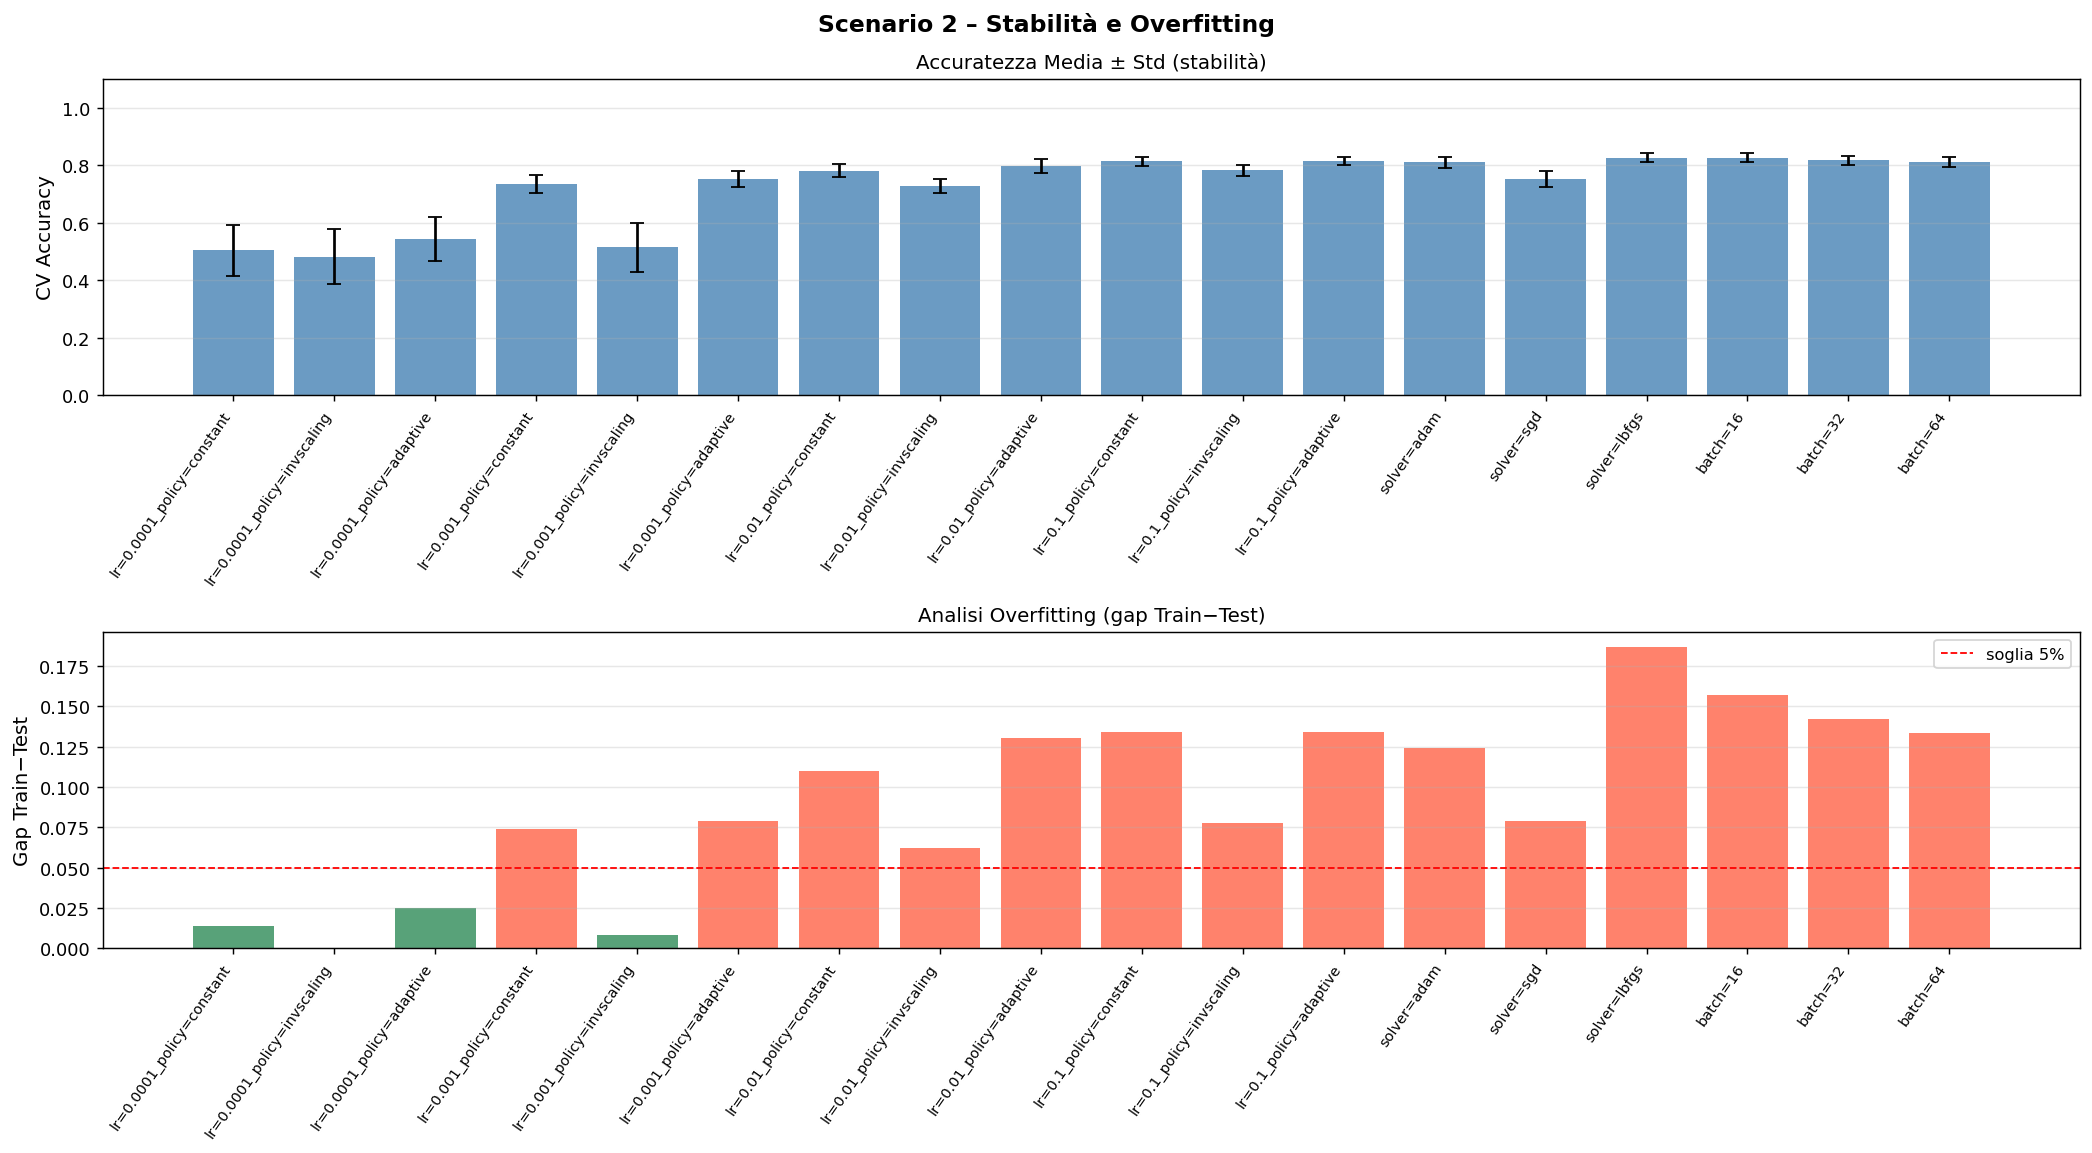
\includegraphics[width=\linewidth]{s2_stability.png}
  \caption{Scenario 2 -- Stabilità (sopra) e analisi overfitting (sotto).}
  \label{fig:s2_stab}
\end{figure}
 
\paragraph{Osservazioni.}
\begin{itemize}[leftmargin=*]
  \item \textbf{Alta instabilità per lr basso}: le prime cinque
        configurazioni ($lr \leq 0.001$) mostrano error bar molto grandi
        (fino a $\pm 0.10$), evidenziando che l'esito dell'addestramento
        dipende fortemente dal seed e dall'inizializzazione quando il LR
        è insufficiente.
  \item Le configurazioni non convergenti (lr$=0.0001$) hanno un gap
        Train--Test \emph{bassissimo} ($<0.05$), ma non perché
        generalizzino bene: semplicemente il modello non impara né in
        training né in test.
  \item A partire da $lr=0.001$\_\texttt{adaptive} il gap sale sopra
        $0.05$, indicando che la rete inizia a imparare ma produce
        overfitting (gap $\approx 8$--$18\%$ per le configurazioni
        convergenti).
  \item \textbf{solver=lbfgs} ha il gap più alto ($>18\%$), coerente
        con la tendenza dei metodi quasi-Newton a memorizzare il training
        set su dataset di dimensione moderata.
  \item Tra i batch size, \textbf{batch=64} mostra il gap più contenuto
        ($\approx 13\%$), suggerendo che batch più grandi fungono da
        regolarizzatore implicito.
\end{itemize}
 
\newpage
% =============================================================================
\section{Scenario 3 -- Regolarizzazione ed Early Stopping}
% =============================================================================
 
\subsection{Contesto}
 
Lo Scenario 3 fissa l'architettura $(400,200)$, attivazione \texttt{tanh},
solver \texttt{adam}, $\text{lr}=0.001$ e varia i parametri di
regolarizzazione:
\begin{enumerate}
  \item \textbf{L2 penalty} \texttt{alpha}: $0.0001$, $0.001$, $0.01$,
        $0.1$, $0.5$.
  \item \textbf{Early stopping} on/off.
  \item \textbf{Validation fraction}: $0.10$, $0.15$, $0.20$.
  \item \textbf{n\_iter\_no\_change}: $5$, $10$, $20$.
\end{enumerate}
 
% ─────────────────────────────────────────────────────────────────────────────
\subsection{Box plot dell'accuracy (CV 5-fold)}
 
\begin{figure}[H]
  \centering
  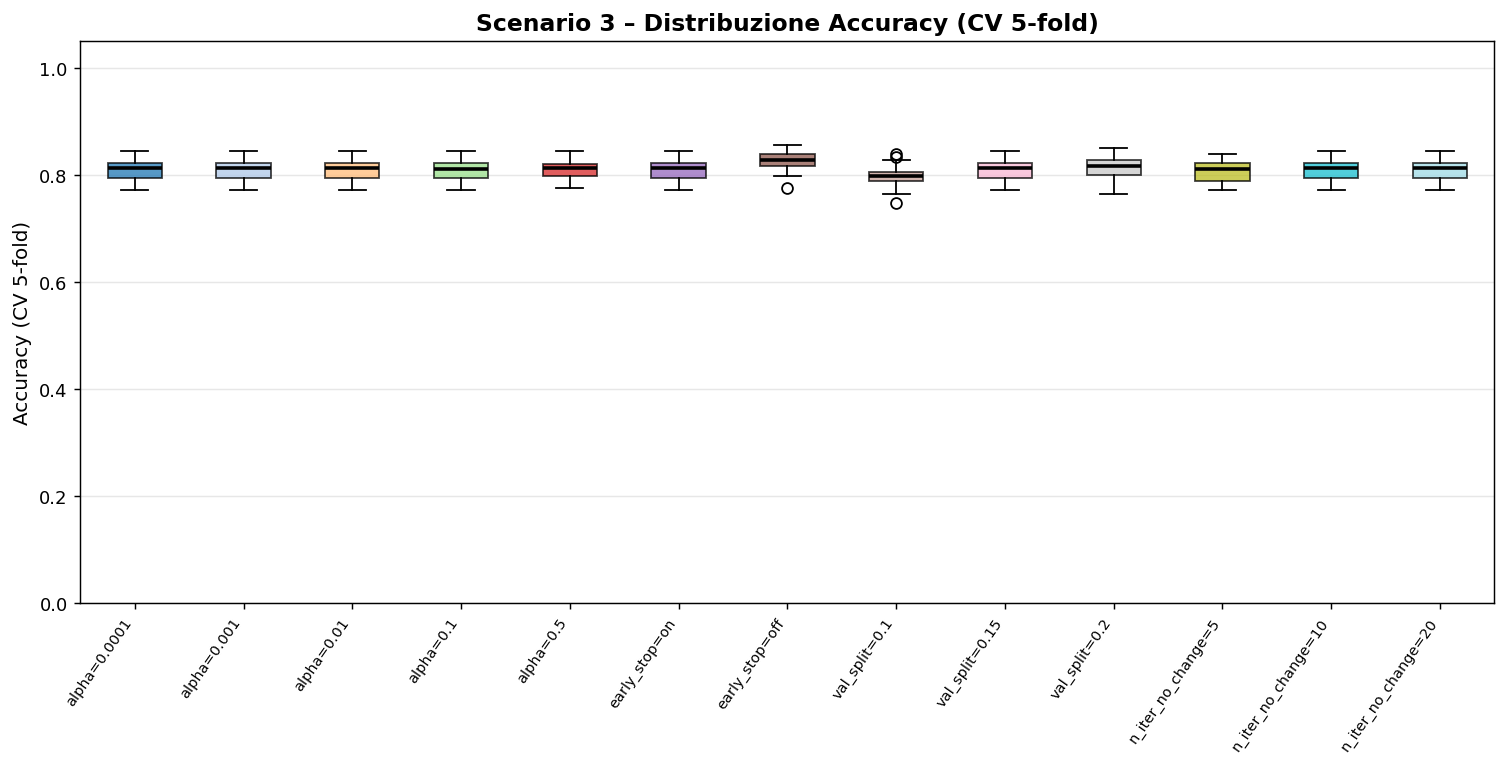
\includegraphics[width=0.9\linewidth]{s3_accuracy_boxplot.png}
  \caption{Scenario 3 -- Distribuzione accuracy CV 5-fold.}
  \label{fig:s3_boxplot}
\end{figure}
 
\paragraph{Osservazioni.}
\begin{itemize}[leftmargin=*]
  \item Questo è il grafico più ``uniforme'' dei tre scenari: tutte le
        configurazioni si attestano attorno a $0.80$--$0.82$, con
        varianza molto ridotta.
  \item Il parametro \texttt{alpha} ha un effetto quasi nullo
        nell'intervallo $0.0001$--$0.1$: le mediane sono praticamente
        identiche. Solo \texttt{alpha=0.5} mostra un lieve decremento
        ($\approx 0.80$), indicando che una penalizzazione così aggressiva
        inizia a costringere eccessivamente i pesi.
  \item \textbf{early\_stop=off} produce la distribuzione con la mediana
        più alta ($\approx 0.82$) ma anche qualche outlier basso: senza
        early stopping la rete può imparare di più ma è meno stabile.
  \item Le variazioni di \texttt{val\_split} e \texttt{n\_iter\_no\_change}
        hanno impatto trascurabile sull'accuracy CV, confermando che
        la configurazione di base è già robusta.
\end{itemize}
 
\begin{tcolorbox}[commentbox]
L'accuracy di questo scenario è la più alta e stabile dei tre. Il dataset
DARWIN è ben appreso da \texttt{(400,200)\_tanh\_adam} indipendentemente
dai dettagli di regolarizzazione, che incidono principalmente
sull'overfitting (vedi Sez.~\ref{sec:s3_stab}).
\end{tcolorbox}
 
% ─────────────────────────────────────────────────────────────────────────────
\subsection{Matrici di confusione (media 30 run)}
 
\begin{figure}[H]
  \centering
  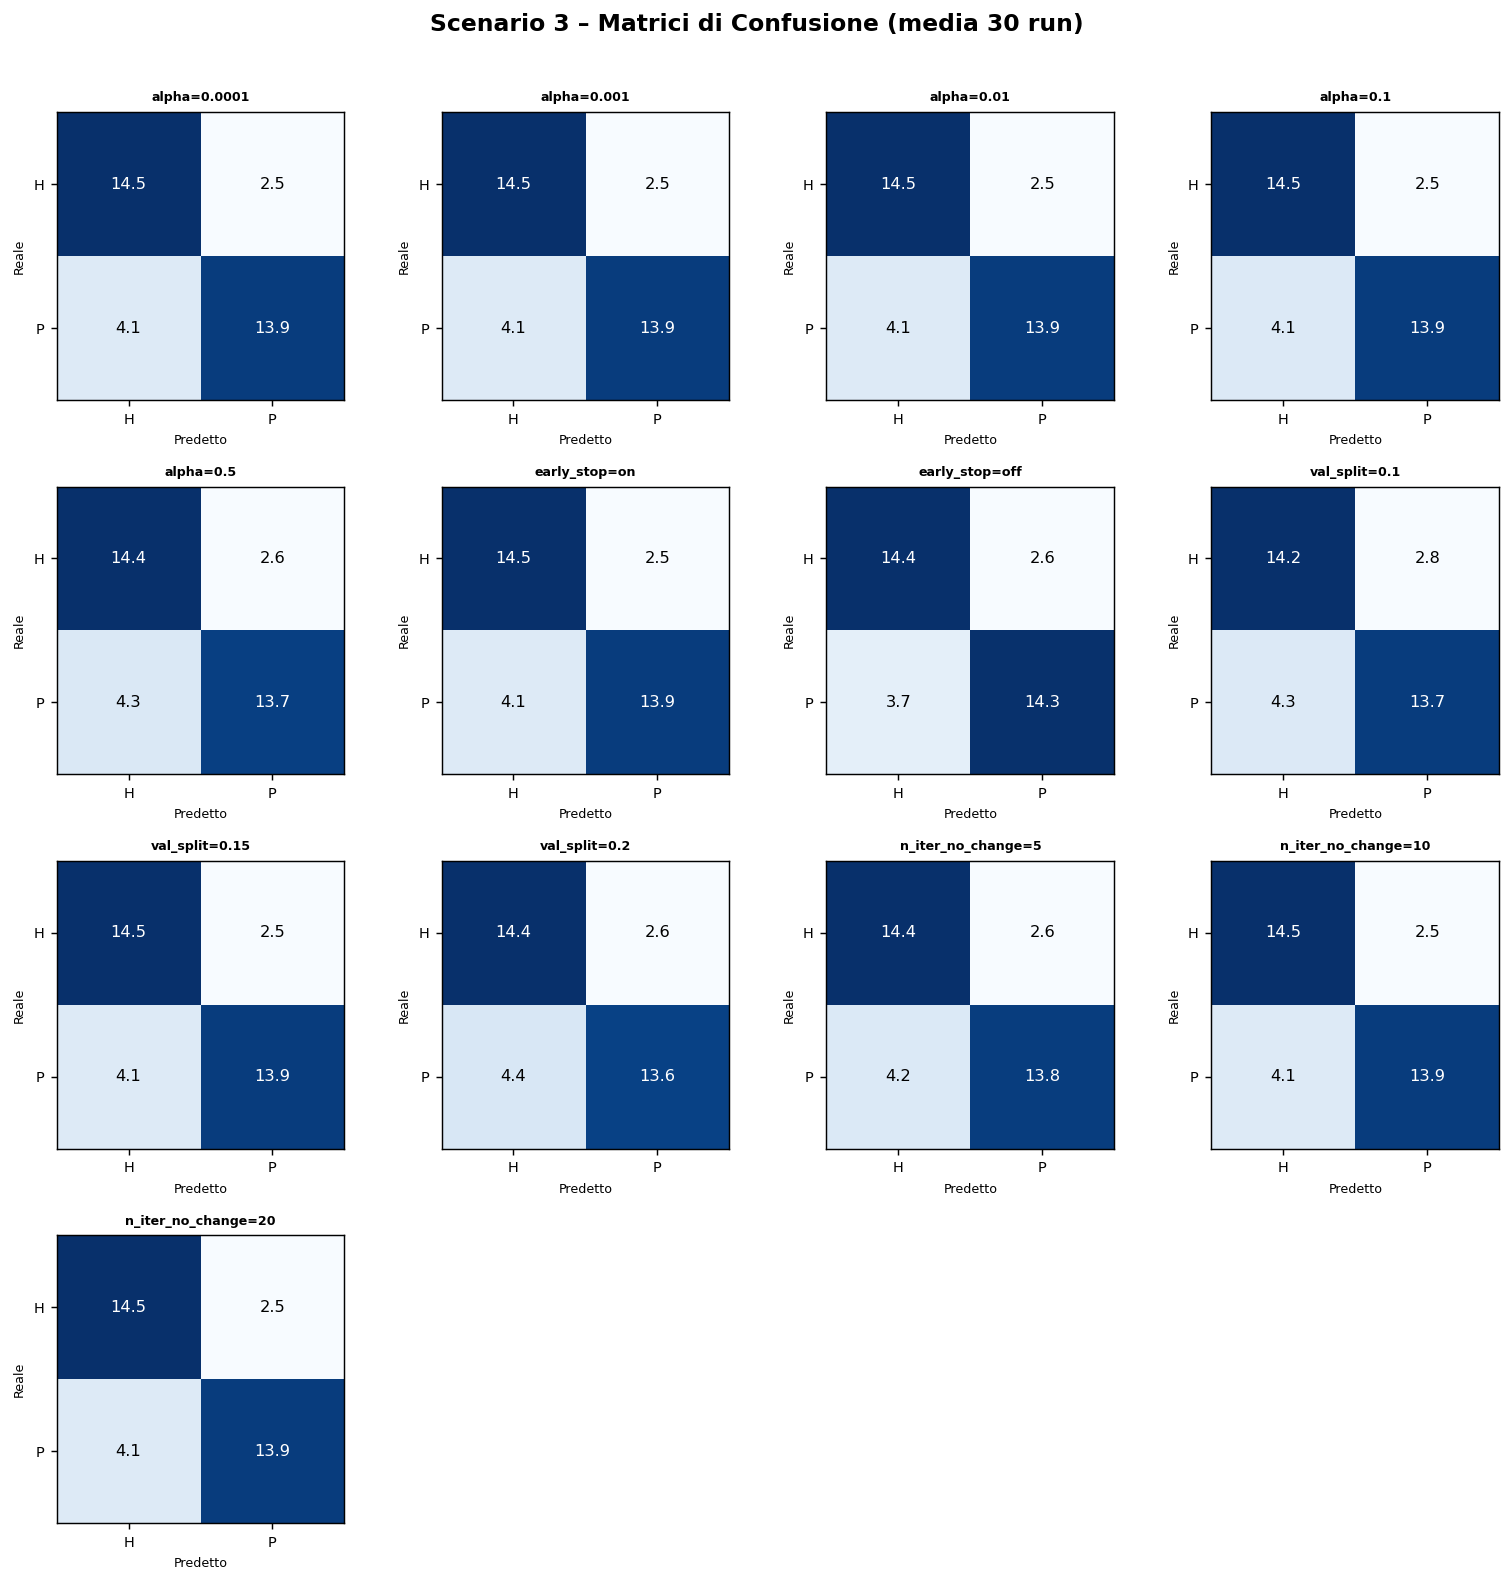
\includegraphics[width=0.85\linewidth]{s3_confusion_matrices.png}
  \caption{Scenario 3 -- Matrici di confusione mediate su 30 run.}
  \label{fig:s3_cm}
\end{figure}
 
\paragraph{Osservazioni.}
\begin{itemize}[leftmargin=*]
  \item Le matrici sono notevolmente stabili tra le configurazioni:
        quasi tutte mostrano $14.4$--$14.5$ TN, $13.7$--$13.9$ TP,
        $2.5$--$2.6$ FP, $4.1$--$4.3$ FN.
  \item La configurazione \textbf{early\_stop=off} si distingue con
        soli $3.7$ FN (il minimo di questo scenario), a costo però di
        maggiore overfitting (vedi analisi successiva).
  \item \textbf{val\_split=0.1} mostra $2.8$ FP (leggermente più alto),
        probabilmente perché la riduzione della frazione di validazione
        altera il criterio di stop precoce.
  \item La stabilità delle matrici conferma che l'architettura e
        l'attivazione dominano le prestazioni, mentre la regolarizzazione
        fine-tuning agisce principalmente sul gap generalization.
\end{itemize}
 
% ─────────────────────────────────────────────────────────────────────────────
\subsection{Curve di apprendimento (Loss)}
 
\begin{figure}[H]
  \centering
  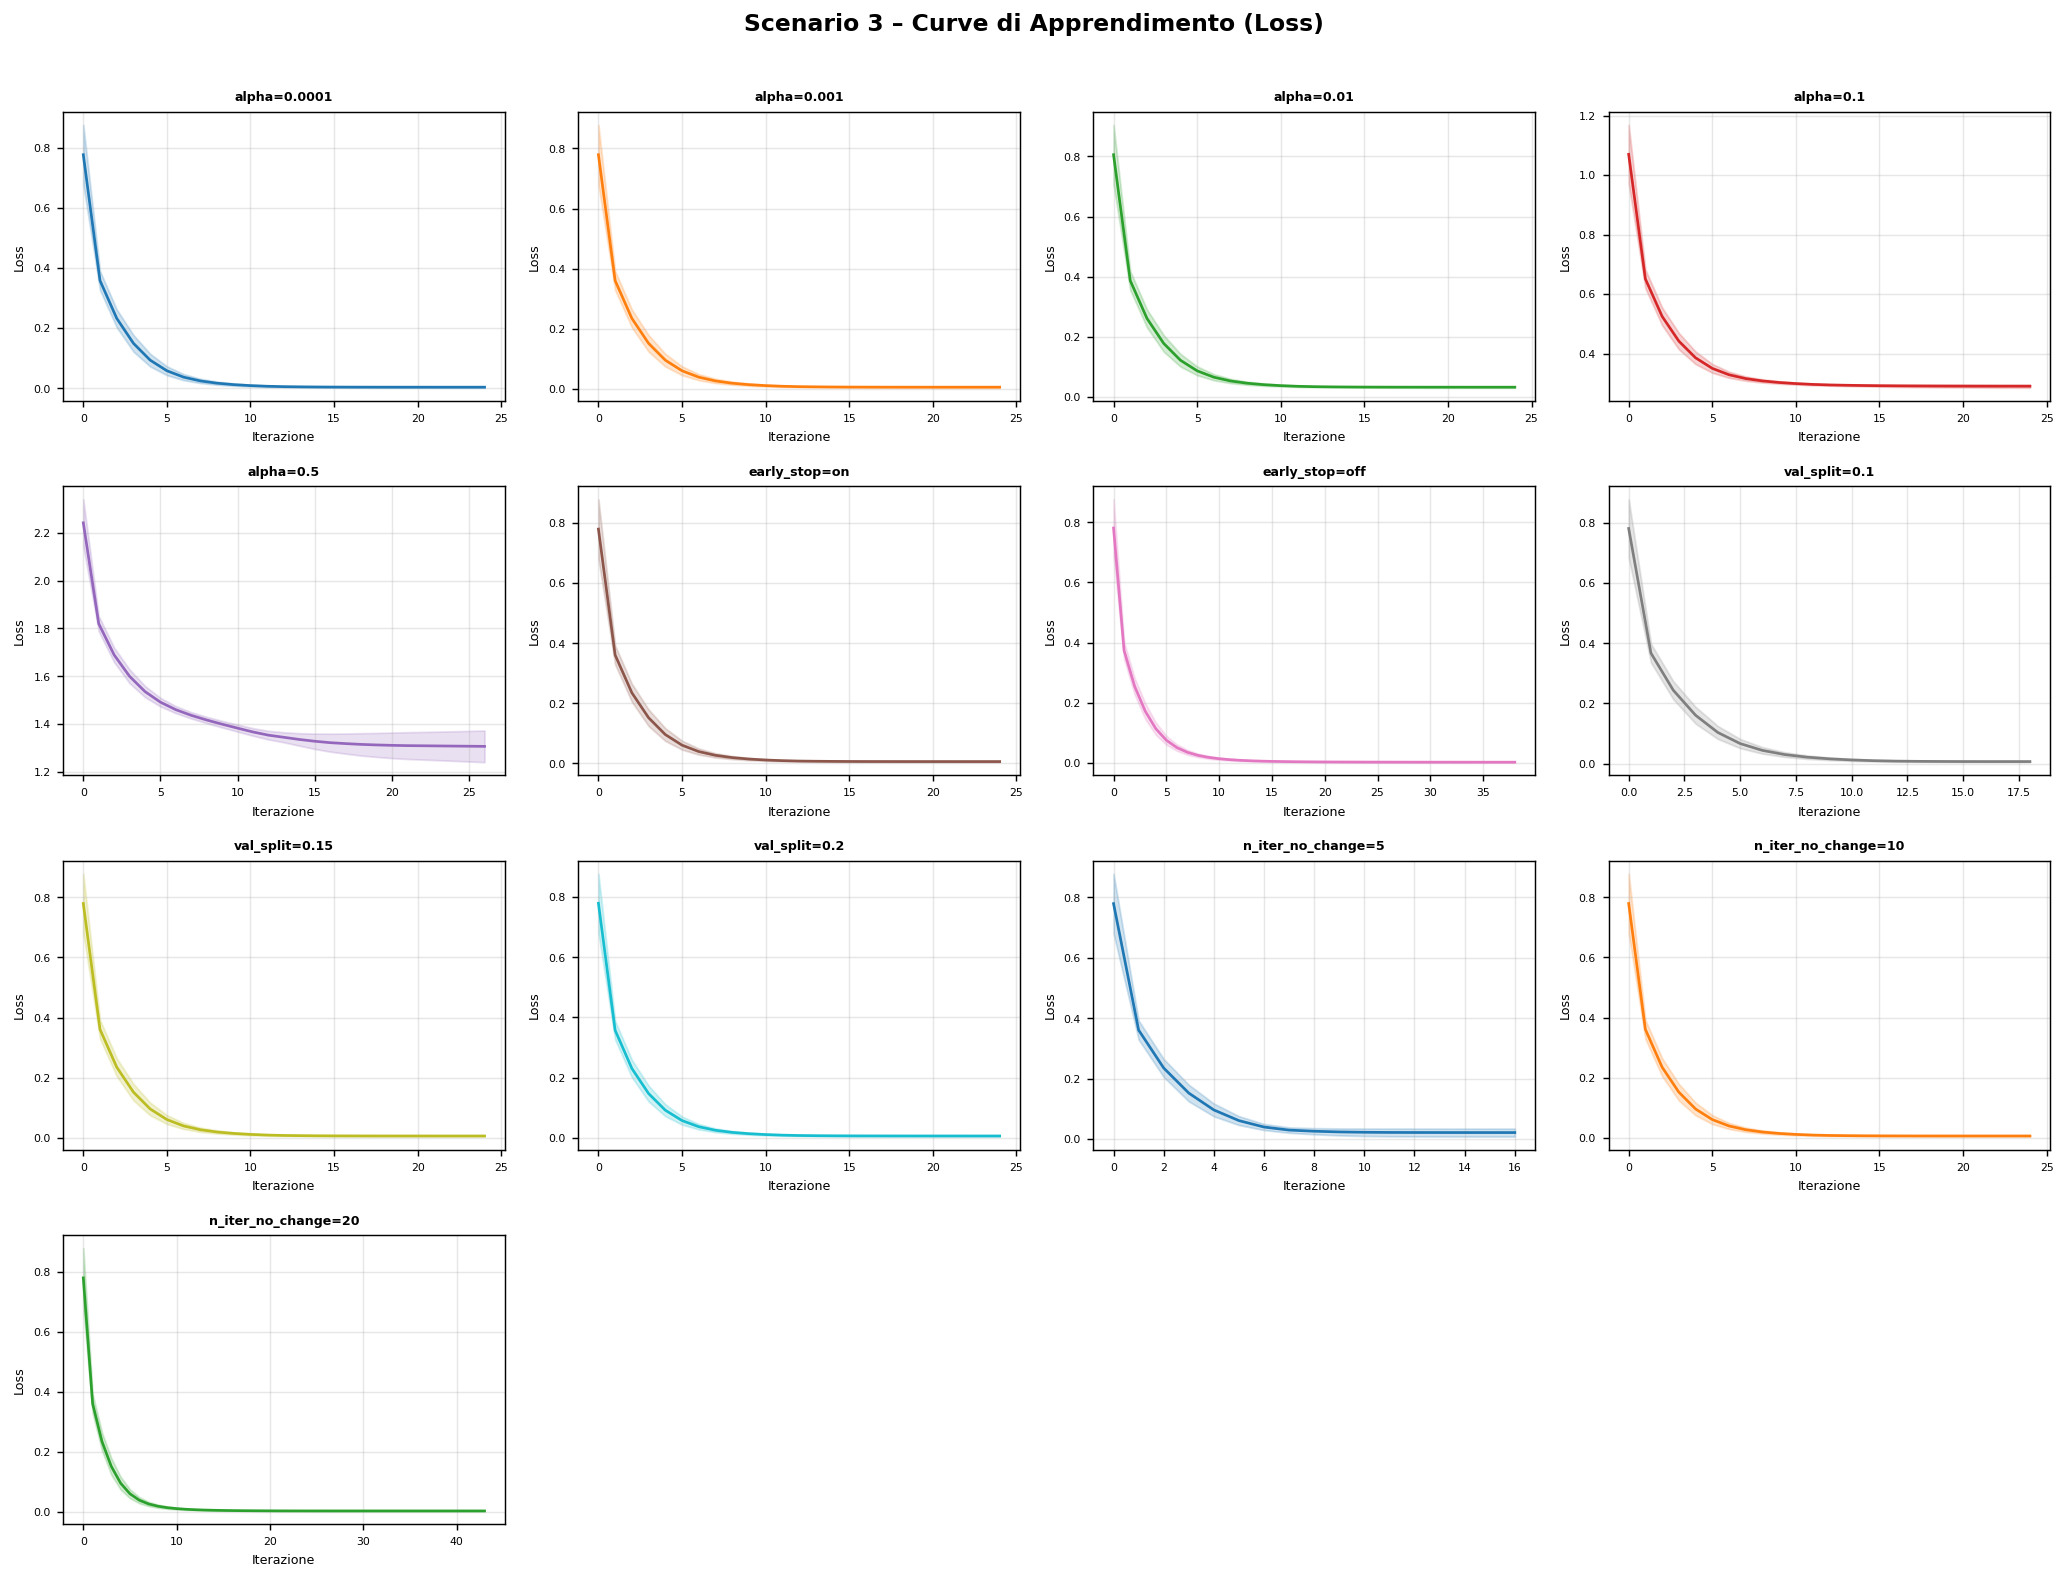
\includegraphics[width=0.95\linewidth]{s3_learning_curves.png}
  \caption{Scenario 3 -- Curve di apprendimento (loss media $\pm$ std).}
  \label{fig:s3_lc}
\end{figure}
 
\paragraph{Osservazioni.}
\begin{itemize}[leftmargin=*]
  \item Per \texttt{alpha} nell'intervallo $0.0001$--$0.1$, le curve sono
        praticamente sovrapponibili: decrescita rapida nelle prime
        5--10 iterazioni, poi convergenza a loss $\approx 0.03$--$0.05$.
  \item \textbf{\texttt{alpha=0.5}} mostra una loss iniziale molto più
        alta ($\approx 2.3$) e converge a un plateau più elevato
        ($\approx 1.25$), confermando che la penalizzazione L2 aggressiva
        limita la capacità espressiva della rete.
  \item \textbf{early\_stop=off} produce la curva più lunga (fino a 37
        iterazioni) e raggiunge la loss finale più bassa, confermando
        che senza il criterio di arresto precoce la rete continua a
        ottimizzare il training set.
  \item \textbf{n\_iter\_no\_change=5} arresta il training molto presto
        (solo 16 iterazioni in media), giustificando il tempo di
        esecuzione ridotto osservato nel box plot dei tempi.
  \item Le bande di deviazione standard sono strettissime in tutto lo
        Scenario 3, evidenziando la massima riproducibilità di questa
        configurazione base.
\end{itemize}
 
% ─────────────────────────────────────────────────────────────────────────────
\subsection{Curve ROC}
 
\begin{figure}[H]
  \centering
  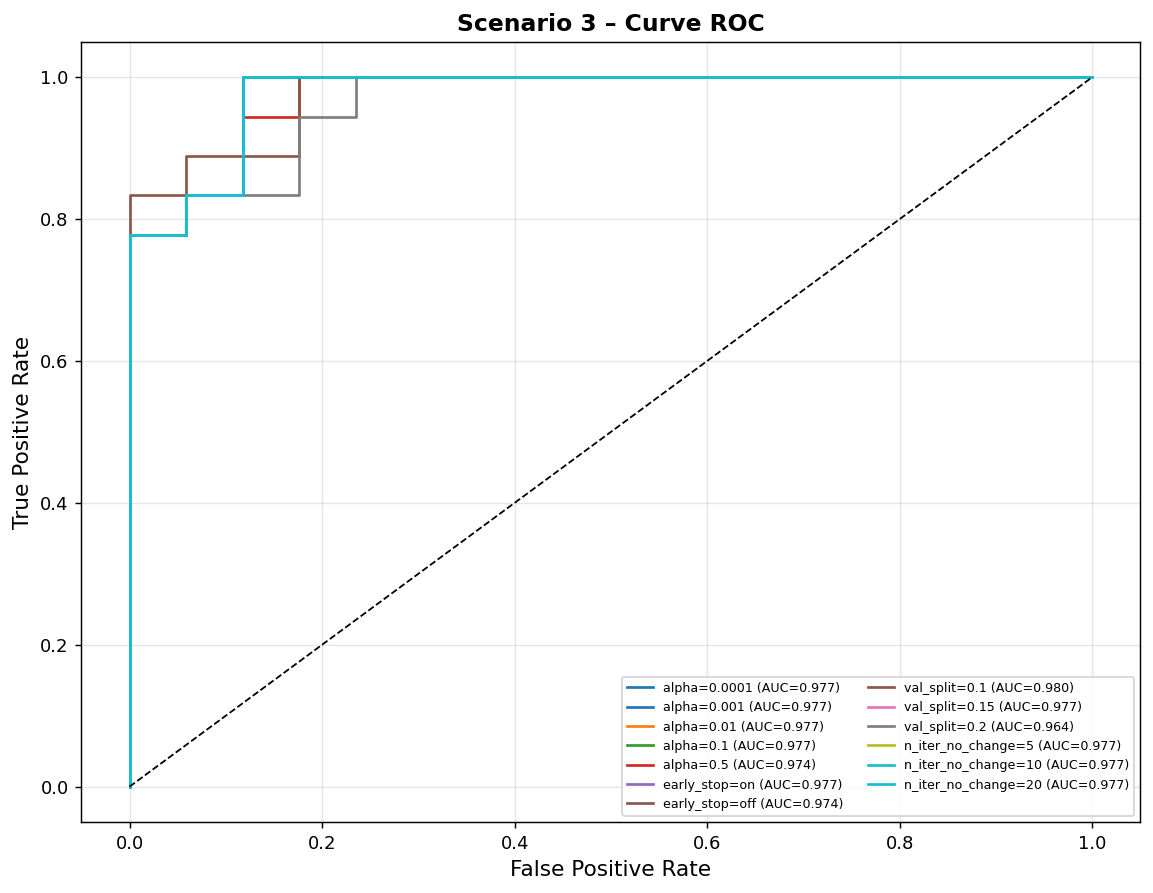
\includegraphics[width=0.8\linewidth]{s3_roc_curves.png}
  \caption{Scenario 3 -- Curve ROC (best run per configurazione).}
  \label{fig:s3_roc}
\end{figure}
 
\paragraph{Osservazioni.}
\begin{itemize}[leftmargin=*]
  \item Le AUC variano nel ristretto intervallo $0.964$--$0.980$,
        il gruppo più compatto dei tre scenari.
  \item \textbf{val\_split=0.1} ottiene l'AUC più alta ($0.980$),
        forse perché una validation fraction più piccola lascia più
        dati al training, migliorando marginalmente la qualità dei
        pesi finali.
  \item \textbf{val\_split=0.2} ha l'AUC più bassa ($0.964$),
        coerentemente con il ragionamento opposto.
  \item Le curve ROC si sovrappongono quasi perfettamente, confermando
        che la capacità discriminativa del modello è insensibile
        alle variazioni di regolarizzazione nel range testato.
\end{itemize}
 
% ─────────────────────────────────────────────────────────────────────────────
\subsection{Tempi di esecuzione}
 
\begin{figure}[H]
  \centering
  
\includegraphics[width=0.9\linewidth]{s3_exec_time.png}
  \caption{Scenario 3 -- Tempi di esecuzione (secondi).}
  \label{fig:s3_time}
\end{figure}
 
\paragraph{Osservazioni.}
\begin{itemize}[leftmargin=*]
  \item I tempi sono generalmente bassi e omogenei ($0.13$--$0.29$~s),
        con qualche outlier per $\alpha=0.0001$ e $\alpha=0.001$ (fino
        a $0.41$~s).
  \item \textbf{early\_stop=off} è il più lento ($\approx 0.29$~s in
        mediana): senza criterio di arresto la rete percorre tutte le
        iterazioni disponibili.
  \item \textbf{n\_iter\_no\_change=5} è il più rapido ($\approx 0.09$~s
        in mediana), poiché il training si arresta appena la loss smette
        di migliorare per 5 iterazioni consecutive.
  \item \textbf{n\_iter\_no\_change=20} è più lento ($\approx 0.23$~s):
        il training aspetta più a lungo prima di fermarsi, permettendo
        affinamenti più profondi.
\end{itemize}
 
% ─────────────────────────────────────────────────────────────────────────────
\subsection{Stabilità e Overfitting}
\label{sec:s3_stab}
 
\begin{figure}[H]
  \centering
  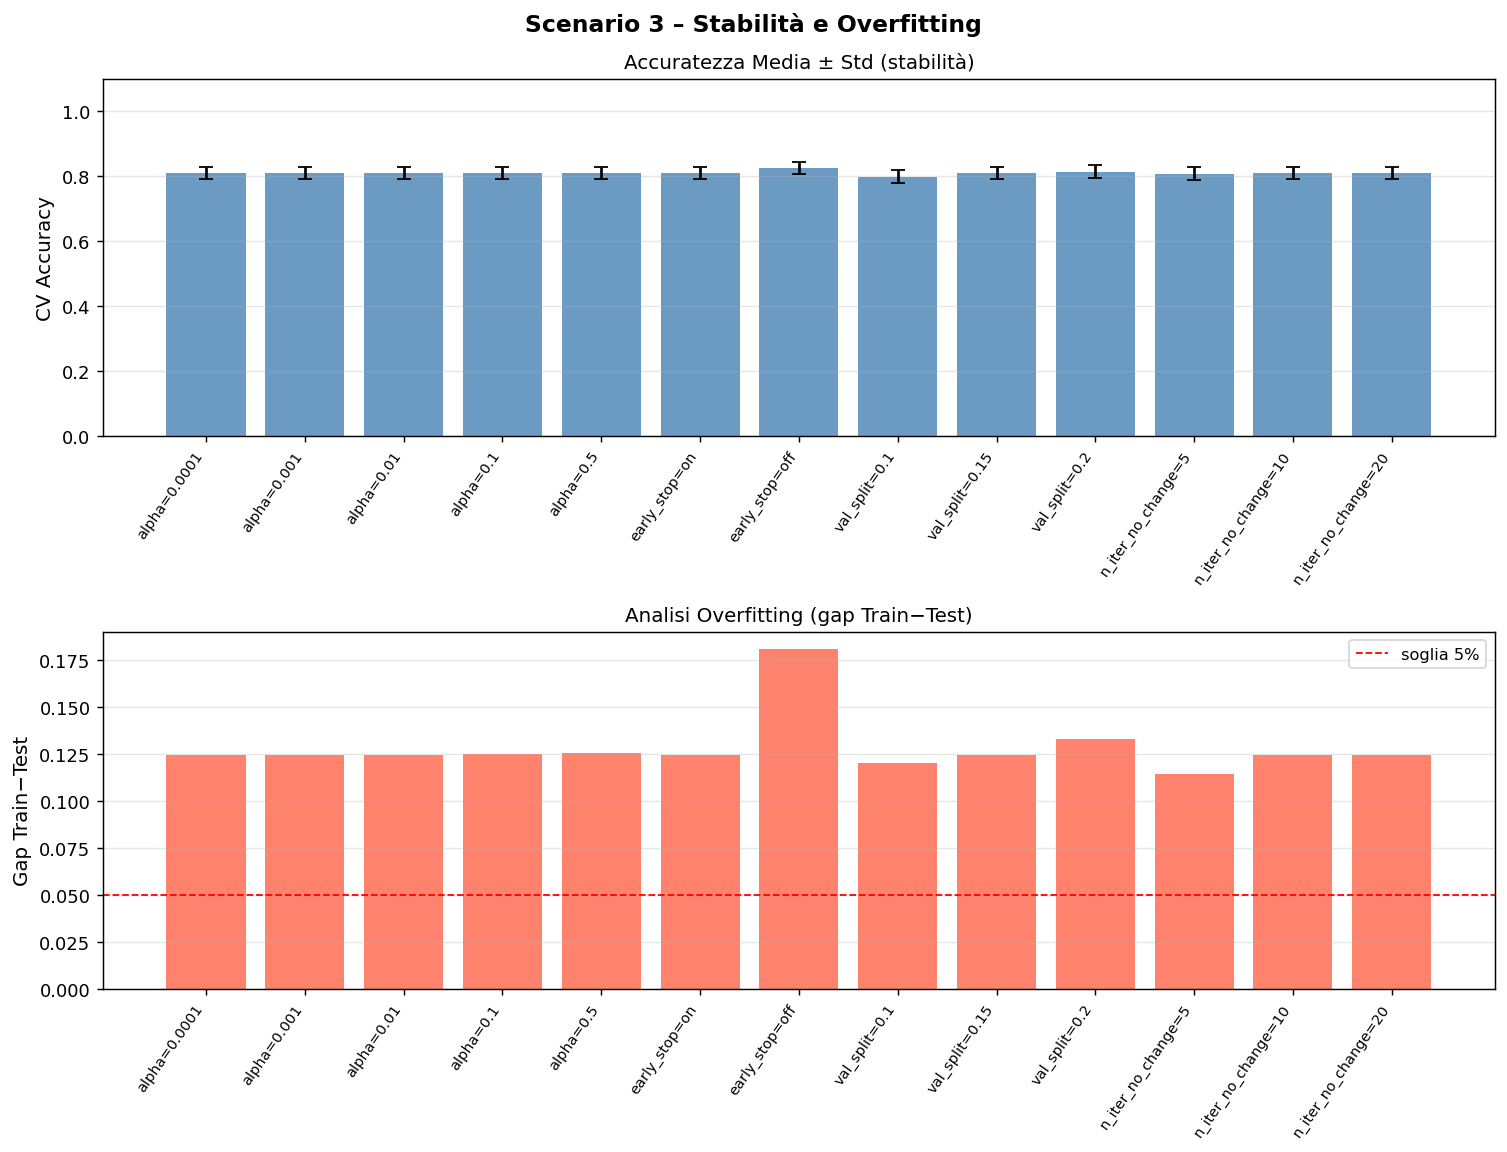
\includegraphics[width=\linewidth]{s3_stability.png}
  \caption{Scenario 3 -- Stabilità (sopra) e analisi overfitting (sotto).}
  \label{fig:s3_stab}
\end{figure}
 
\paragraph{Osservazioni.}
\begin{itemize}[leftmargin=*]
  \item Il pannello superiore conferma l'elevata stabilità: tutte le
        barre sfiorano $0.81$ con error bar $< 0.02$, indipendentemente
        dalla configurazione di regolarizzazione.
  \item Nel pannello inferiore, tutte le configurazioni superano la
        soglia del 5\%, con gap tipici di $\approx 12$--$13\%$.
  \item \textbf{early\_stop=off} produce il gap più alto ($\approx 18\%$):
        senza early stopping la rete si adatta eccessivamente al training,
        confermando l'utilità del criterio di arresto precoce per
        il controllo dell'overfitting.
  \item L'aumento di \texttt{alpha} da $0.0001$ a $0.5$ non riduce
        significativamente il gap, suggerendo che per questo dataset
        e questa architettura la regolarizzazione L2 non è lo strumento
        principale di controllo dell'overfitting nell'intervallo esplorato.
  \item \textbf{n\_iter\_no\_change=5} mostra il gap più basso tra le
        varianti di early stopping ($\approx 11\%$): terminare prima il
        training riduce la memorizzazione.
\end{itemize}
 
\begin{tcolorbox}[commentbox]
Nello Scenario 3 il fattore che impatta maggiormente l'overfitting è la
presenza/assenza dell'early stopping, non il valore di \texttt{alpha} o
di \texttt{val\_split}. Abilitare l'early stopping con
\texttt{n\_iter\_no\_change} $\leq 10$ è la strategia di regolarizzazione
più efficace per questo problema.
\end{tcolorbox}
 
\section{Conclusioni}
% =============================================================================
\subsection{Confronto Comparativo tra Scenari}
% =============================================================================
 
La Tabella~\ref{tab:confronto} riassume le migliori configurazioni per
ciascun scenario secondo i criteri principali.
 
\begin{table}[H]
\centering
\caption{Confronto delle migliori configurazioni per scenario.}
\label{tab:confronto}
\begin{tabular}{llcccc}
\toprule
\textbf{Scenario} & \textbf{Migliore config.} & \textbf{CV Acc.} &
\textbf{AUC} & \textbf{Gap OF} & \textbf{Tempo~(s)}\\
\midrule
S1 -- Architettura & $(600,)$\_tanh       & $\approx 0.82$ & $0.997$ & $\approx 10\%$ & $\approx 0.15$ \\
S2 -- LR/Solver    & batch=16 (adam)      & $\approx 0.83$ & $0.987$ & $\approx 15\%$ & $\approx 0.60$ \\
S3 -- Regulariz.   & early\_stop=off      & $\approx 0.83$ & $0.974$ & $\approx 18\%$ & $\approx 0.29$ \\
\midrule
S3 -- Regol.       & alpha=0.01, ES on    & $\approx 0.81$ & $0.977$ & $\approx 12\%$ & $\approx 0.15$ \\
\bottomrule
\end{tabular}
\end{table}
 
\subsection{Considerazioni finali.}
\begin{itemize}[leftmargin=*]
  \item L'\textbf{architettura} impatta principalmente sulla velocità di
        convergenza e sulla minima loss raggiungibile, non sull'accuracy
        CV finale che rimane in un range ristretto.
  \item Il \textbf{learning rate} è il parametro più critico: valori
        inadeguati rendono il training inutilizzabile.
  \item La \textbf{regolarizzazione} (L2 + early stopping) è essenziale
        per ridurre l'overfitting: pur non migliorando l'accuracy CV,
        migliora la generalizzazione.
  \item La configurazione \textbf{raccomandabile} complessiva è:
        architettura $(400,200)$ o $(600,300)$, attivazione \texttt{tanh}
        o \texttt{relu}, solver \texttt{adam} con $\text{lr}=0.001$,
        $\alpha=0.001$, early stopping attivo con \texttt{val\_split=0.15}
        e \texttt{n\_iter\_no\_change=10}. Questa configurazione
        bilancia accuracy ($\approx 0.81$), AUC ($\approx 0.98$),
        overfitting contenuto ($\approx 12\%$) e tempi ragionevoli
        ($\approx 0.15$~s).
\end{itemize}

\end{document}
